
\section{The $\mu$RWell technology}
\label{section:Muon-uRWell}


The $\mu$RWell is a compact, spark-protected and single amplification stage MPGD.
In the $\mu$RWell technology an additional discharge resilience with respect to the triple-GEM detectors is foreseen as well as a simplified assembly geometry.  
A $\mu$RWell detector~\cite{urwell} is composed of two PCBs: a standard GEM Drift PCB acting as the cathode and a $\mu$RWell PCB that couples in a unique structure the electron amplification (a WELL patterned matrix) and the readout stages~\ref{fig:urwell-sketch}a). 
A standard GEM 50 $\mu$m polyimide foil is copper clad on one side and Diamond Like Carbon (DLC) sputtered on the opposite side. 
The thickness of the DLC layer is adjusted according to the desired surface resistivity value (50-200 M$\Omega$/$\Box$) and represents the bottom of the WELL matrix providing discharge suppression as well as current evacuation. 
The foil is then coupled to a readout board~\ref{fig:urwell-sketch}b). 
A chemical etching process is then performed on the top surface of the overall structure in order to create the WELL pattern (conical channels 70 um (50 um) top (bottom) in diameter and 140 $\mu$m pitch) that constitutes the amplification stage~\ref{fig:urwell-sketch}c).  
The high voltage applied between the copper and the resistive DLC layers produces the required electric field within the WELLs that is necessary to develop charge amplification. 
The signal is capacitively collected at the readout strips/pads.
Two main schemes for the resistive layer can be envisaged:  a \textit{low-rate} scheme ( for particles fluxes lower than  100 kHz/cm$^2$) based on a simple resistive layer of suitable resistivity; and an \textit{high-rate} scheme  (for a particle flux up to 1MHz/cm$^2$) based on two resistive layers intra-connected by vias and connected to ground through the readout electrodes.  
%Due to the particles rates expected in the region of the GE21 detector the low- rate configuration is here considered.  
Finally, a drift thickness of 3-4 mm allows for reaching a full efficiency while maintaining a versatile detector compactness. 

%
\begin{figure}[h!]
\centering
\begin{tabular}{cc}
%   \begin{minipage}{0.5\textwidth}
%   \centering
   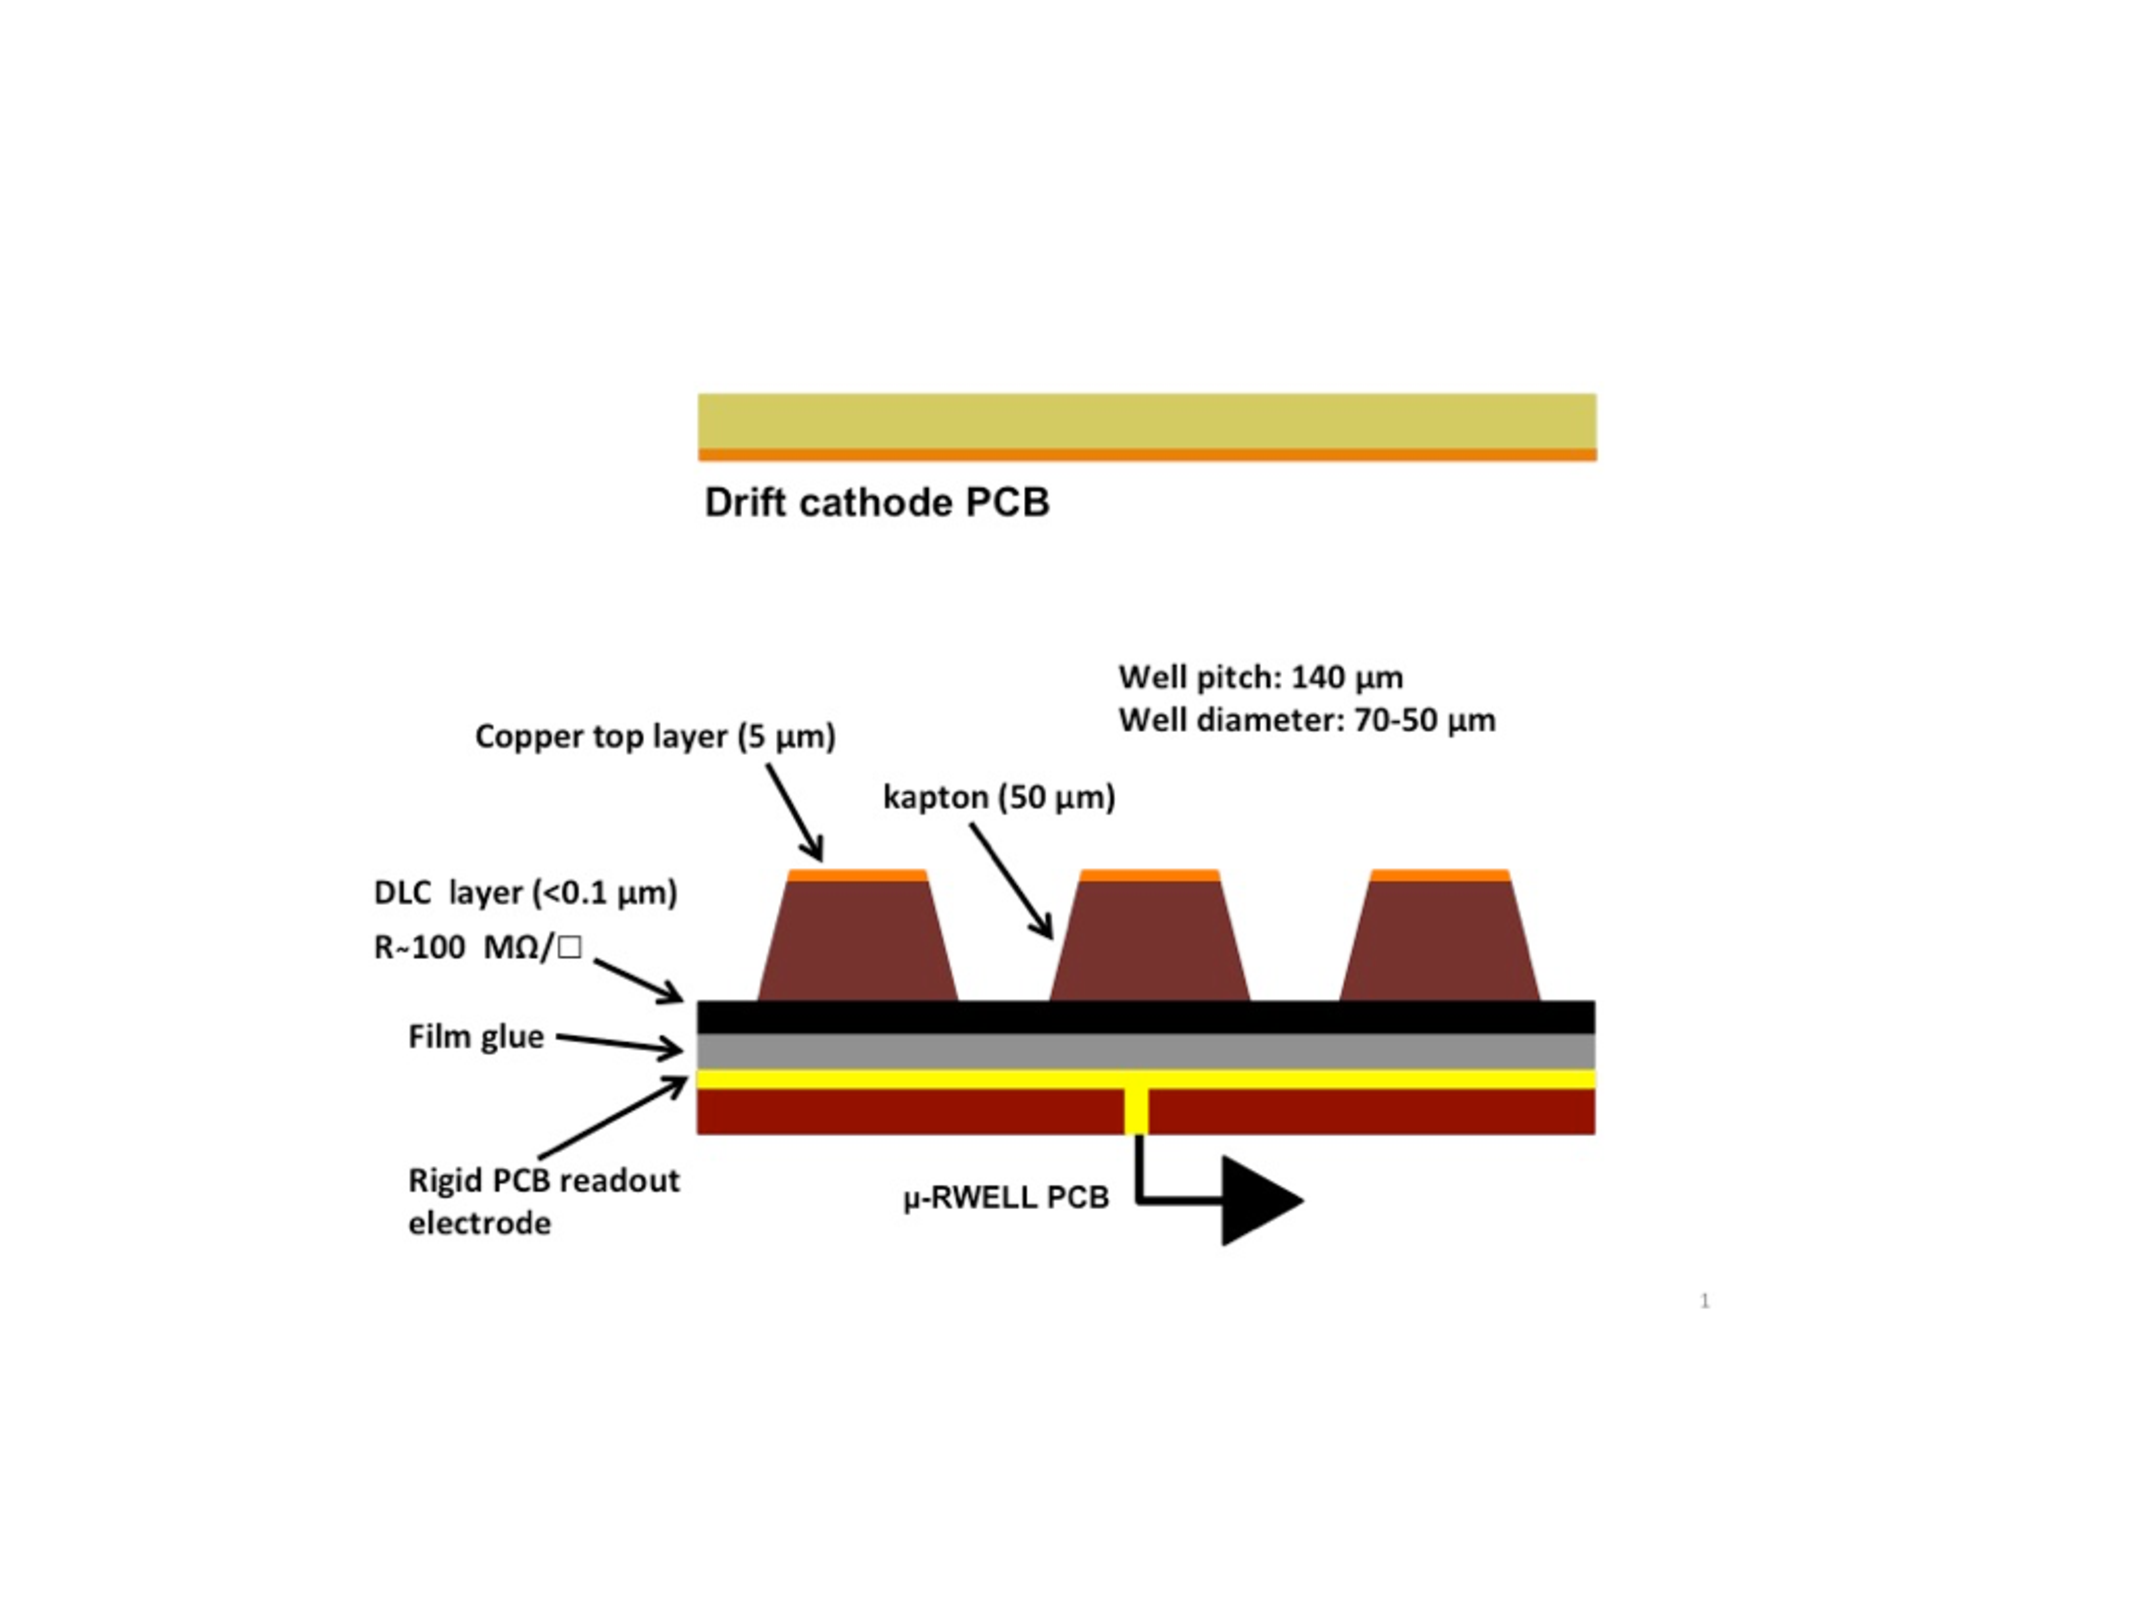
\includegraphics[width=0.5\linewidth]{Figures/Muon/microrwell-sketch.pdf} &
%   \end{minipage}
%   \hfill
%   \begin{minipage}{.5\textwidth}
%   \centering
   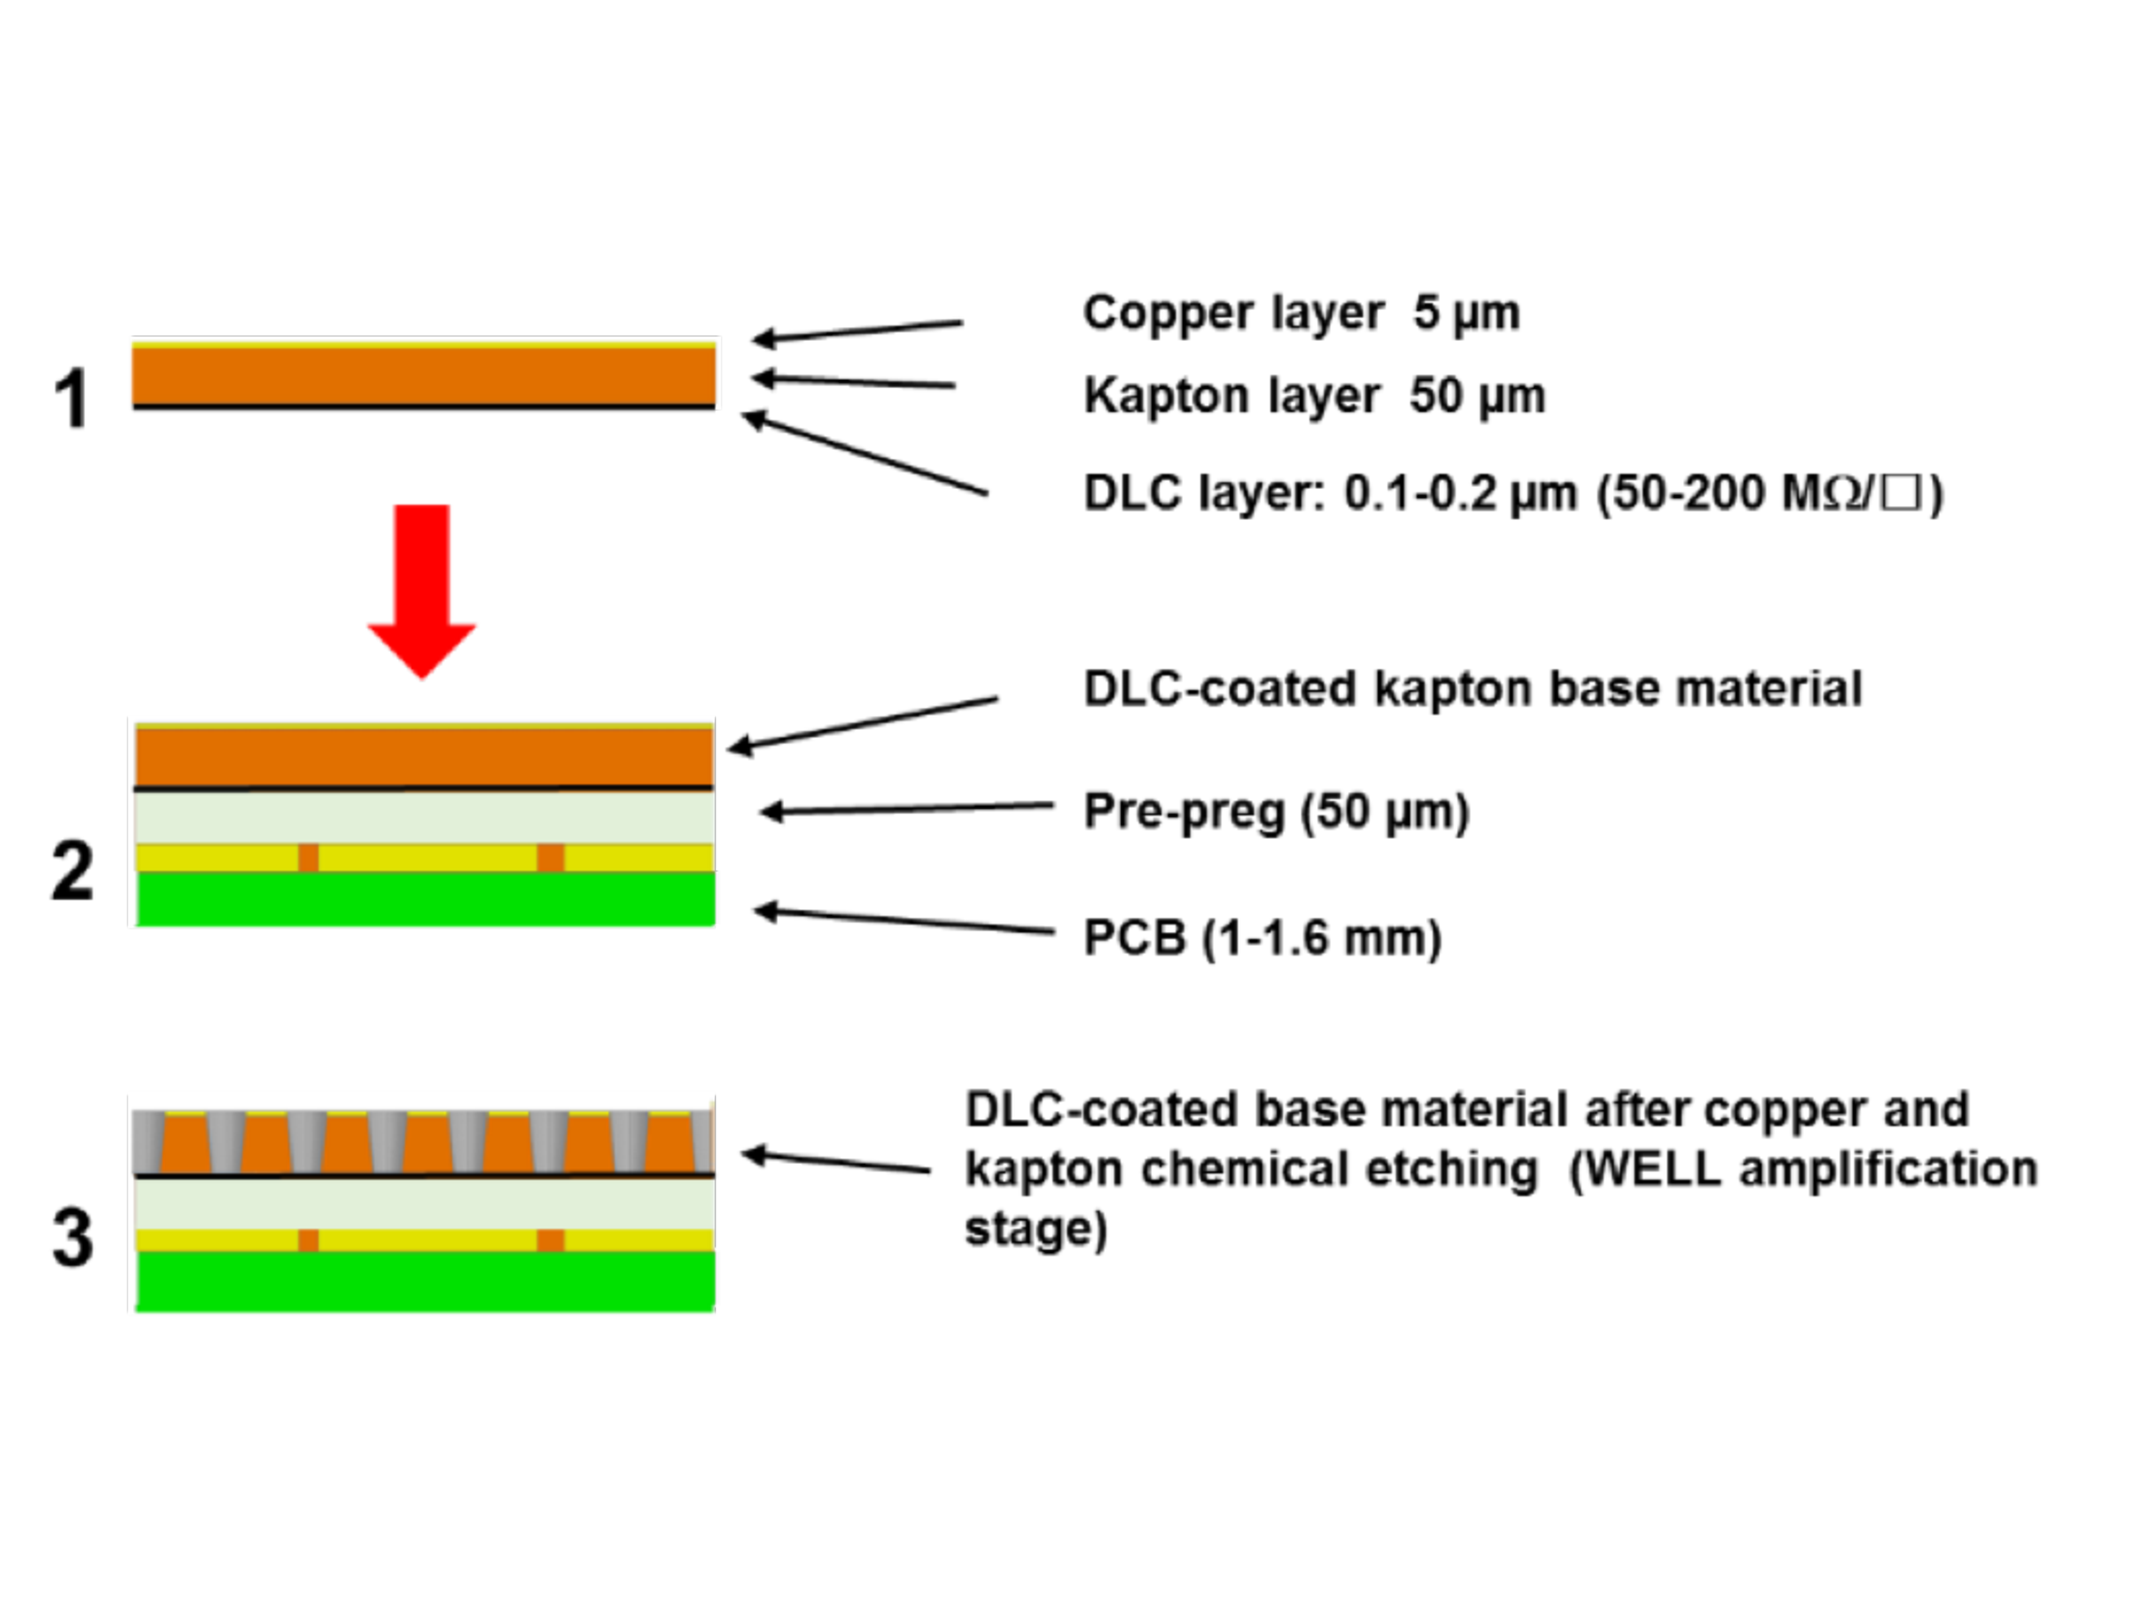
\includegraphics[width=0.5\linewidth]{Figures/Muon/microrwell-sketch-2.pdf} \\
%   \end{minipage}
\end{tabular}
   \vspace{1cm}
   \begin{minipage}{.5\textwidth}
   \centering
   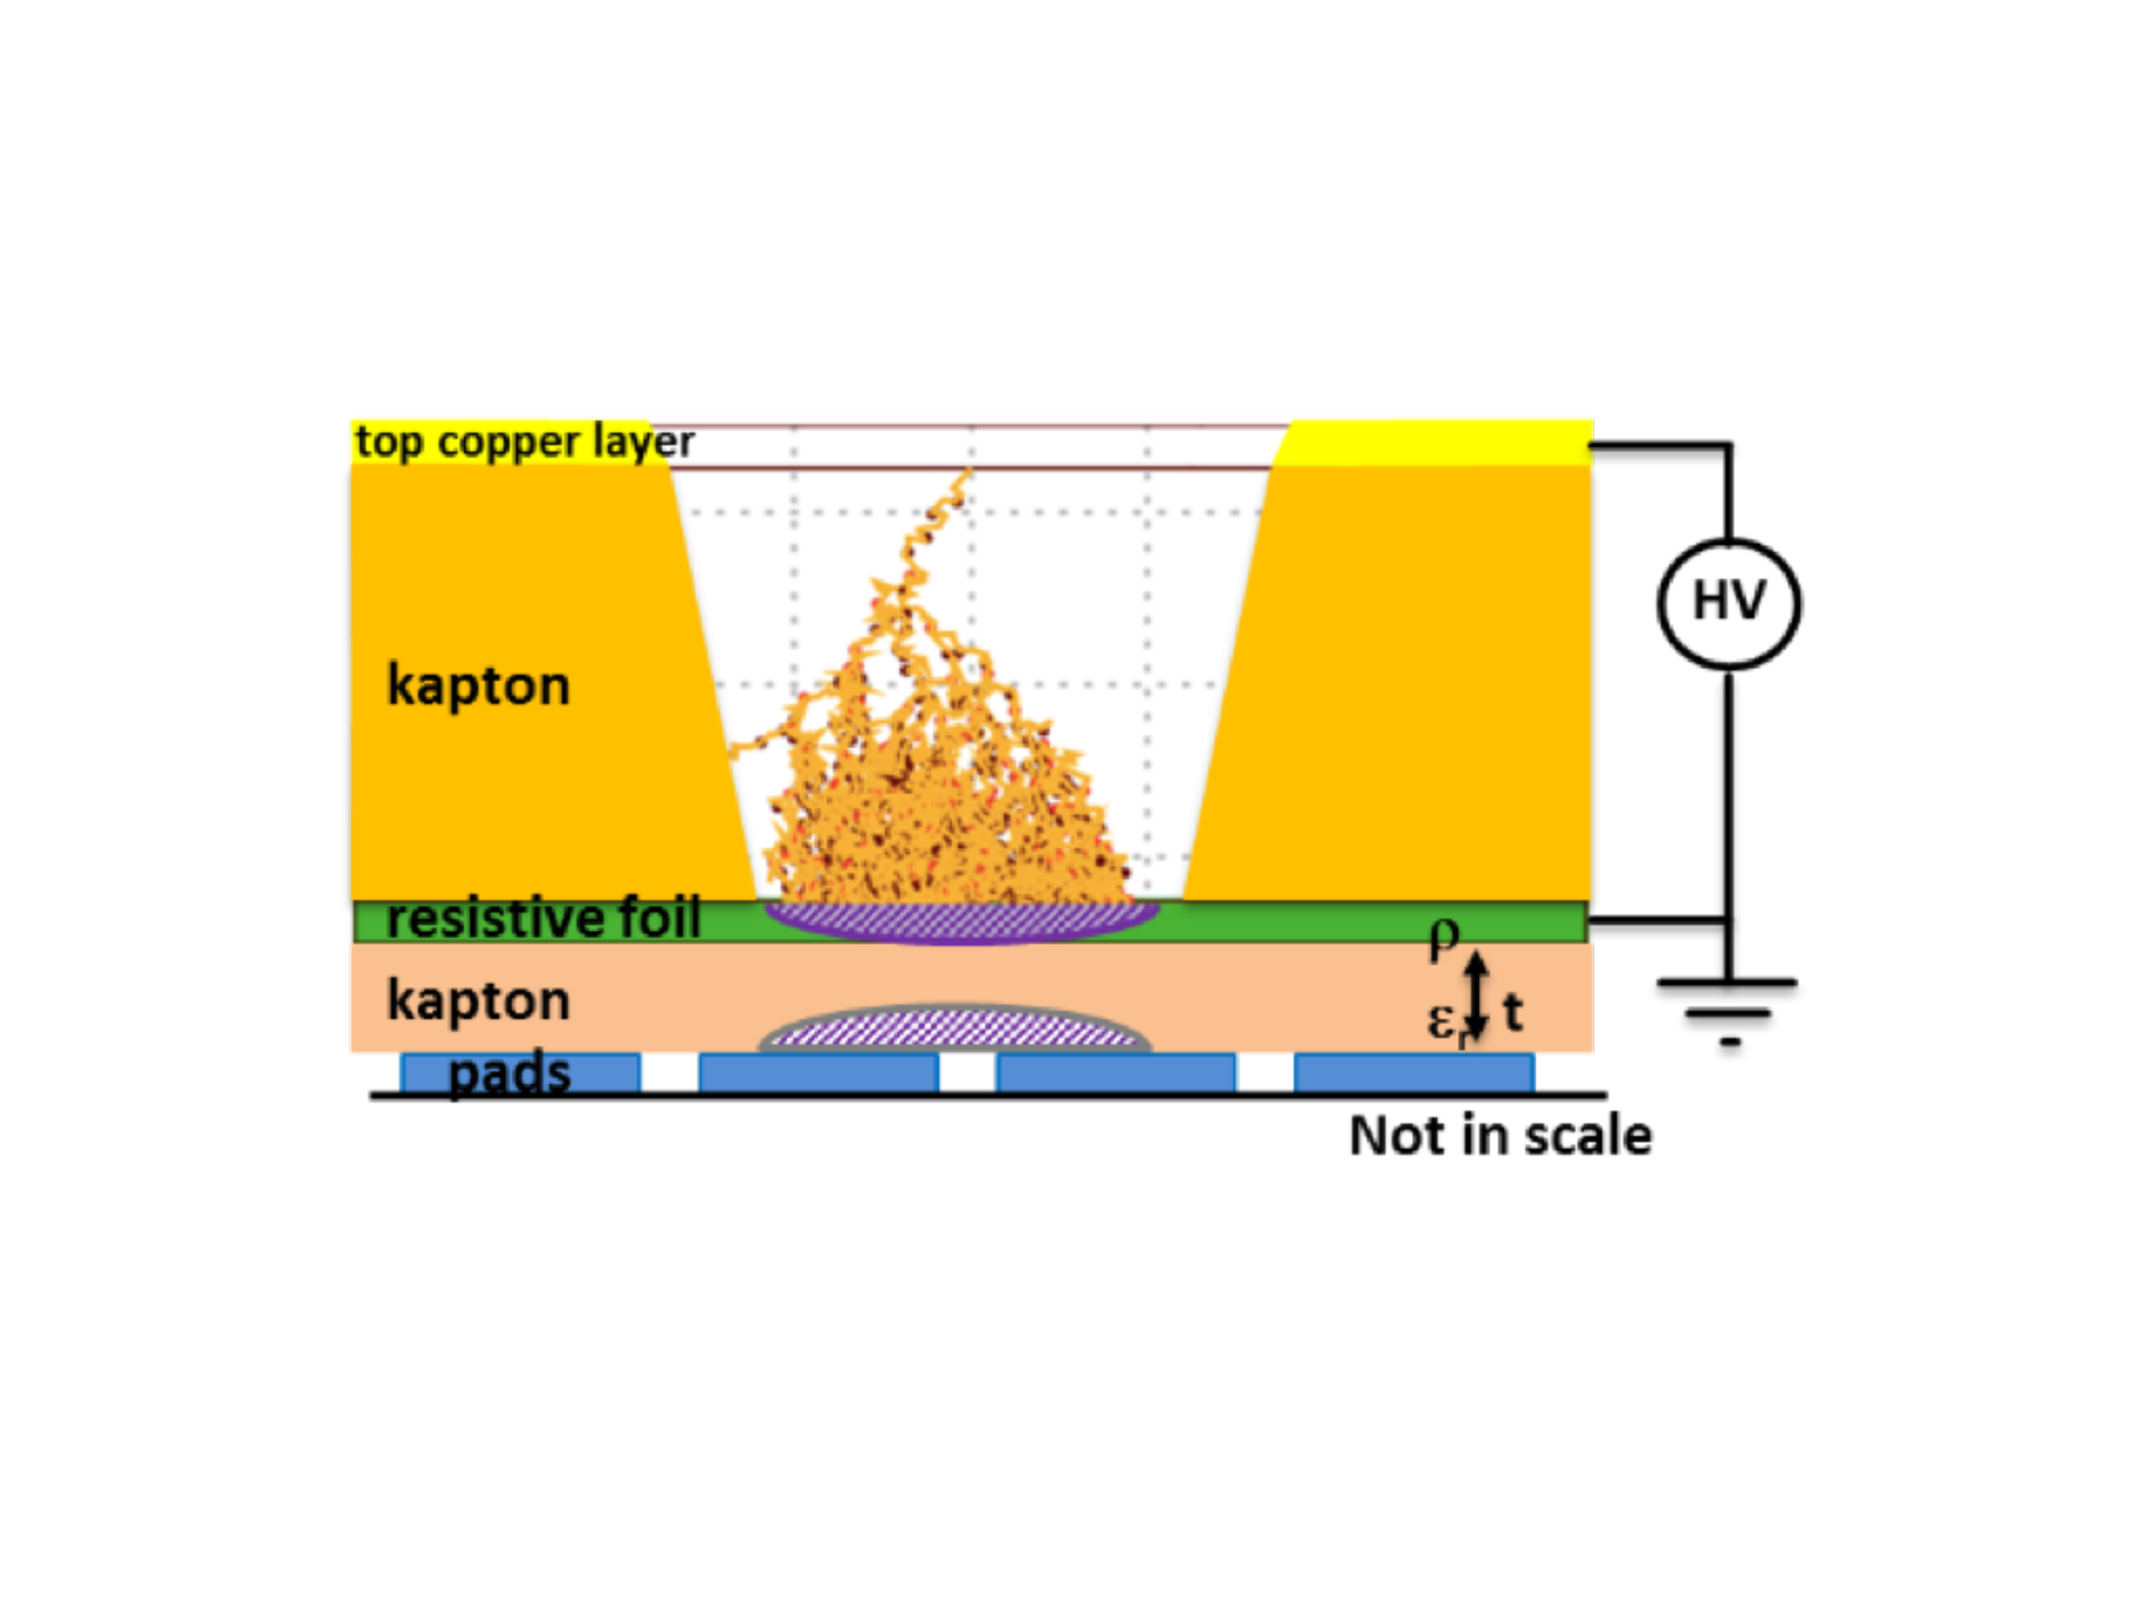
\includegraphics[width=\linewidth]{Figures/Muon/microrwell-sketch-3.pdf}
   \end{minipage}
\caption{a) Layout of a $\mu$RWell detector module; b) Coupling steps of the $\mu$RWell PCB c) Amplification stage directly coupled with the readout. }
\label{fig:urwell-sketch}
\end{figure}


A distinctive advantage of the proposed $\mu$RWell technology is that the detector does not require complex and time-consuming assembly procedures (neither stretching nor gluing), and is definitely much simpler than many other existing MPGDs, such as GEMs or MicroMegas. 
Being composed of only two main components, the cathode and anode PCBs, is extremely simple to be assembled. 
The engineering and the following industrialization of the u-RWell technology is one of the most important goals of the project.
The engineering of the detector essentially coincides with the technological transfer of the manufacturing process of the anode PCB to a suitable industrial partner. 
The main advantage of the $\mu$RWell technology with respect to other MPGD technologies (such as GEM or MM) is that in principle most of the manufacturing steps are already available by a typical company working on rigid and flexible PCB technology. 
In particular, the anode PCB manufacturing, apart from the DLC coating and the etching of the holes on the thin polyimide foil, the technology and the know-how are already available at the ELTOS Company (an Italian company located in the industrial area around Arezzo, specialized in rigid PCB).
While the DLC dry sputtering will probably still be performed by a specialized external company (at the moment this is done by a Japanese firm), the polyimide etching to realize the micro-hole pattern, currently in the hand of the PCB-Workshop of CERN, will be the object of a technological transfer to the industrial partner.
The technology is suitable for large area tracking devices and compact digital hadron calorimetry in HEP experiments; for X-ray and neutron imaging in industrial applications, medical and in particular for homeland security, where muon tomography requires very large area coverage.
The technology could also be a much better option to cope with the more stringent requirements introduced in future experimental scenarios by dealing with those high luminosity high energy beams foreseen in the next generation particle accelerators, as CEPC or FCC.


\subsection{Prototypes performance}
\label{sec:performance-single}
%
The gas gain of the detectors has been measured with a collimated flux of 5.9 keV photons generated by an X-ray gun.
The measurement is performed in current mode, by monitoring the current drawn through the resistive layer as a function of the potential applied to the amplification stage.\\
The gas gain of each detector, measured for the Ar:i-C$_{4}$H$_{10}$ 90:10 gas mixture, 
is typically $\geq$ 10000, being stopped when current instabilities are observed: the largest gain seems to be reached with the most resistive detector (fig. \ref{gain}).
%
\begin{figure}
\centering
\begin{minipage}{0.47\textwidth}
\centering
		\vspace{-0.9cm}
%        \includegraphics[width=\textwidth]{gain_final}
        %{Gain_vs_resistivity_fit_BNC}
        \caption{Measured gain for the three detectors.}
        \label{gain}
        \end{minipage}
        \hspace{0.5cm}
 	\begin{minipage}{0.47\textwidth}
    \centering
%    \includegraphics[width=\textwidth]{ariso_ratecapa_12_80_880_blu}	
        \caption{Normalized gain for 12~M$\Omega/\Box$ (blue open squares), 80~M$\Omega/\Box$ (black full circles) and 880~M$\Omega/\Box$ (red empty circles)}
    	\label{ratecapa-single}
	\end{minipage}
\end{figure}
%
The dependence of the rate capability on the resistivity of the various prototypes has been measured at the gain G$\sim$4000 with the usual collimated (2.5 mm diameter) photon X-ray gun.\\
As shown in fig.\ref{ratecapa-single}, the gain decrease is correlated with the voltage drop due to the resistive layer: the higher the DLC resistivity the lower is the rate capability, ranging from few tens of kHz/cm$^2$ up to a few MHz/cm$^2$. 
A more trustworthy measurement of the rate capability achievable with the single-resistive layer configuration of the detector has been obtained irradiating with a $\sim$3x3 cm$^2$ (FWHM) pion beam (see section ~\ref{section:uRWell-performance}) two different sectors of a large area detector with a $\sim$ 70 M$\Omega/\Box$ resistivity (section ~\ref{sec:large-size}). The result, as reported in \cite{NIM-RWELL-1}, indicates that the detector can stand a particle flux above 35 kHz/cm$^2$.\\
The tracking performance of the three prototypes and its dependence on the resistivity of the DLC film has been tested with a muon beam at the H4 line of the SPS test area at CERN.\\
All detectors have been operated in Ar:i-C$_{4}$H$_{10}$ 90:10 and read-out by APV hybrid cards \cite{apv} handled by an SRS system. The APV chip, supplying analog output signals, allows the study of the detector tracking performance based on the charge centroid method.\\
The resistive anodic film is equivalent to a distributed 2-D resistive-capacitive network with respect to the readout plane.
The localized charge produced in the amplification stage of the detector arriving on the resistive anode surface is dispersed with a time constant depending on the surface resistivity and the capacitance per unit area (see section~\ref{sec:intro}).\\
As a consequence the spatial resolution, as shown in fig. \ref{rho_res}, depends on the surface resistivity of the DLC film showing a clear minimum around 100$\div$200 M$\Omega/\Box$.
At low surface resistivity the charge dispersion increases, the distribution loses the typical Gaussian shape and consequently the $\sigma$  becomes larger. At high surface resistivity the charge dispersion is so negligible (the strip cluster size being close to 1 - in strip unit) that the charge centroid method becomes no more effective and the $\sigma$ approaches the limit of pitch/$\sqrt{12}$ (strip pitch = 0.4 mm).\\
%
\begin{figure}[h]
\centering
    	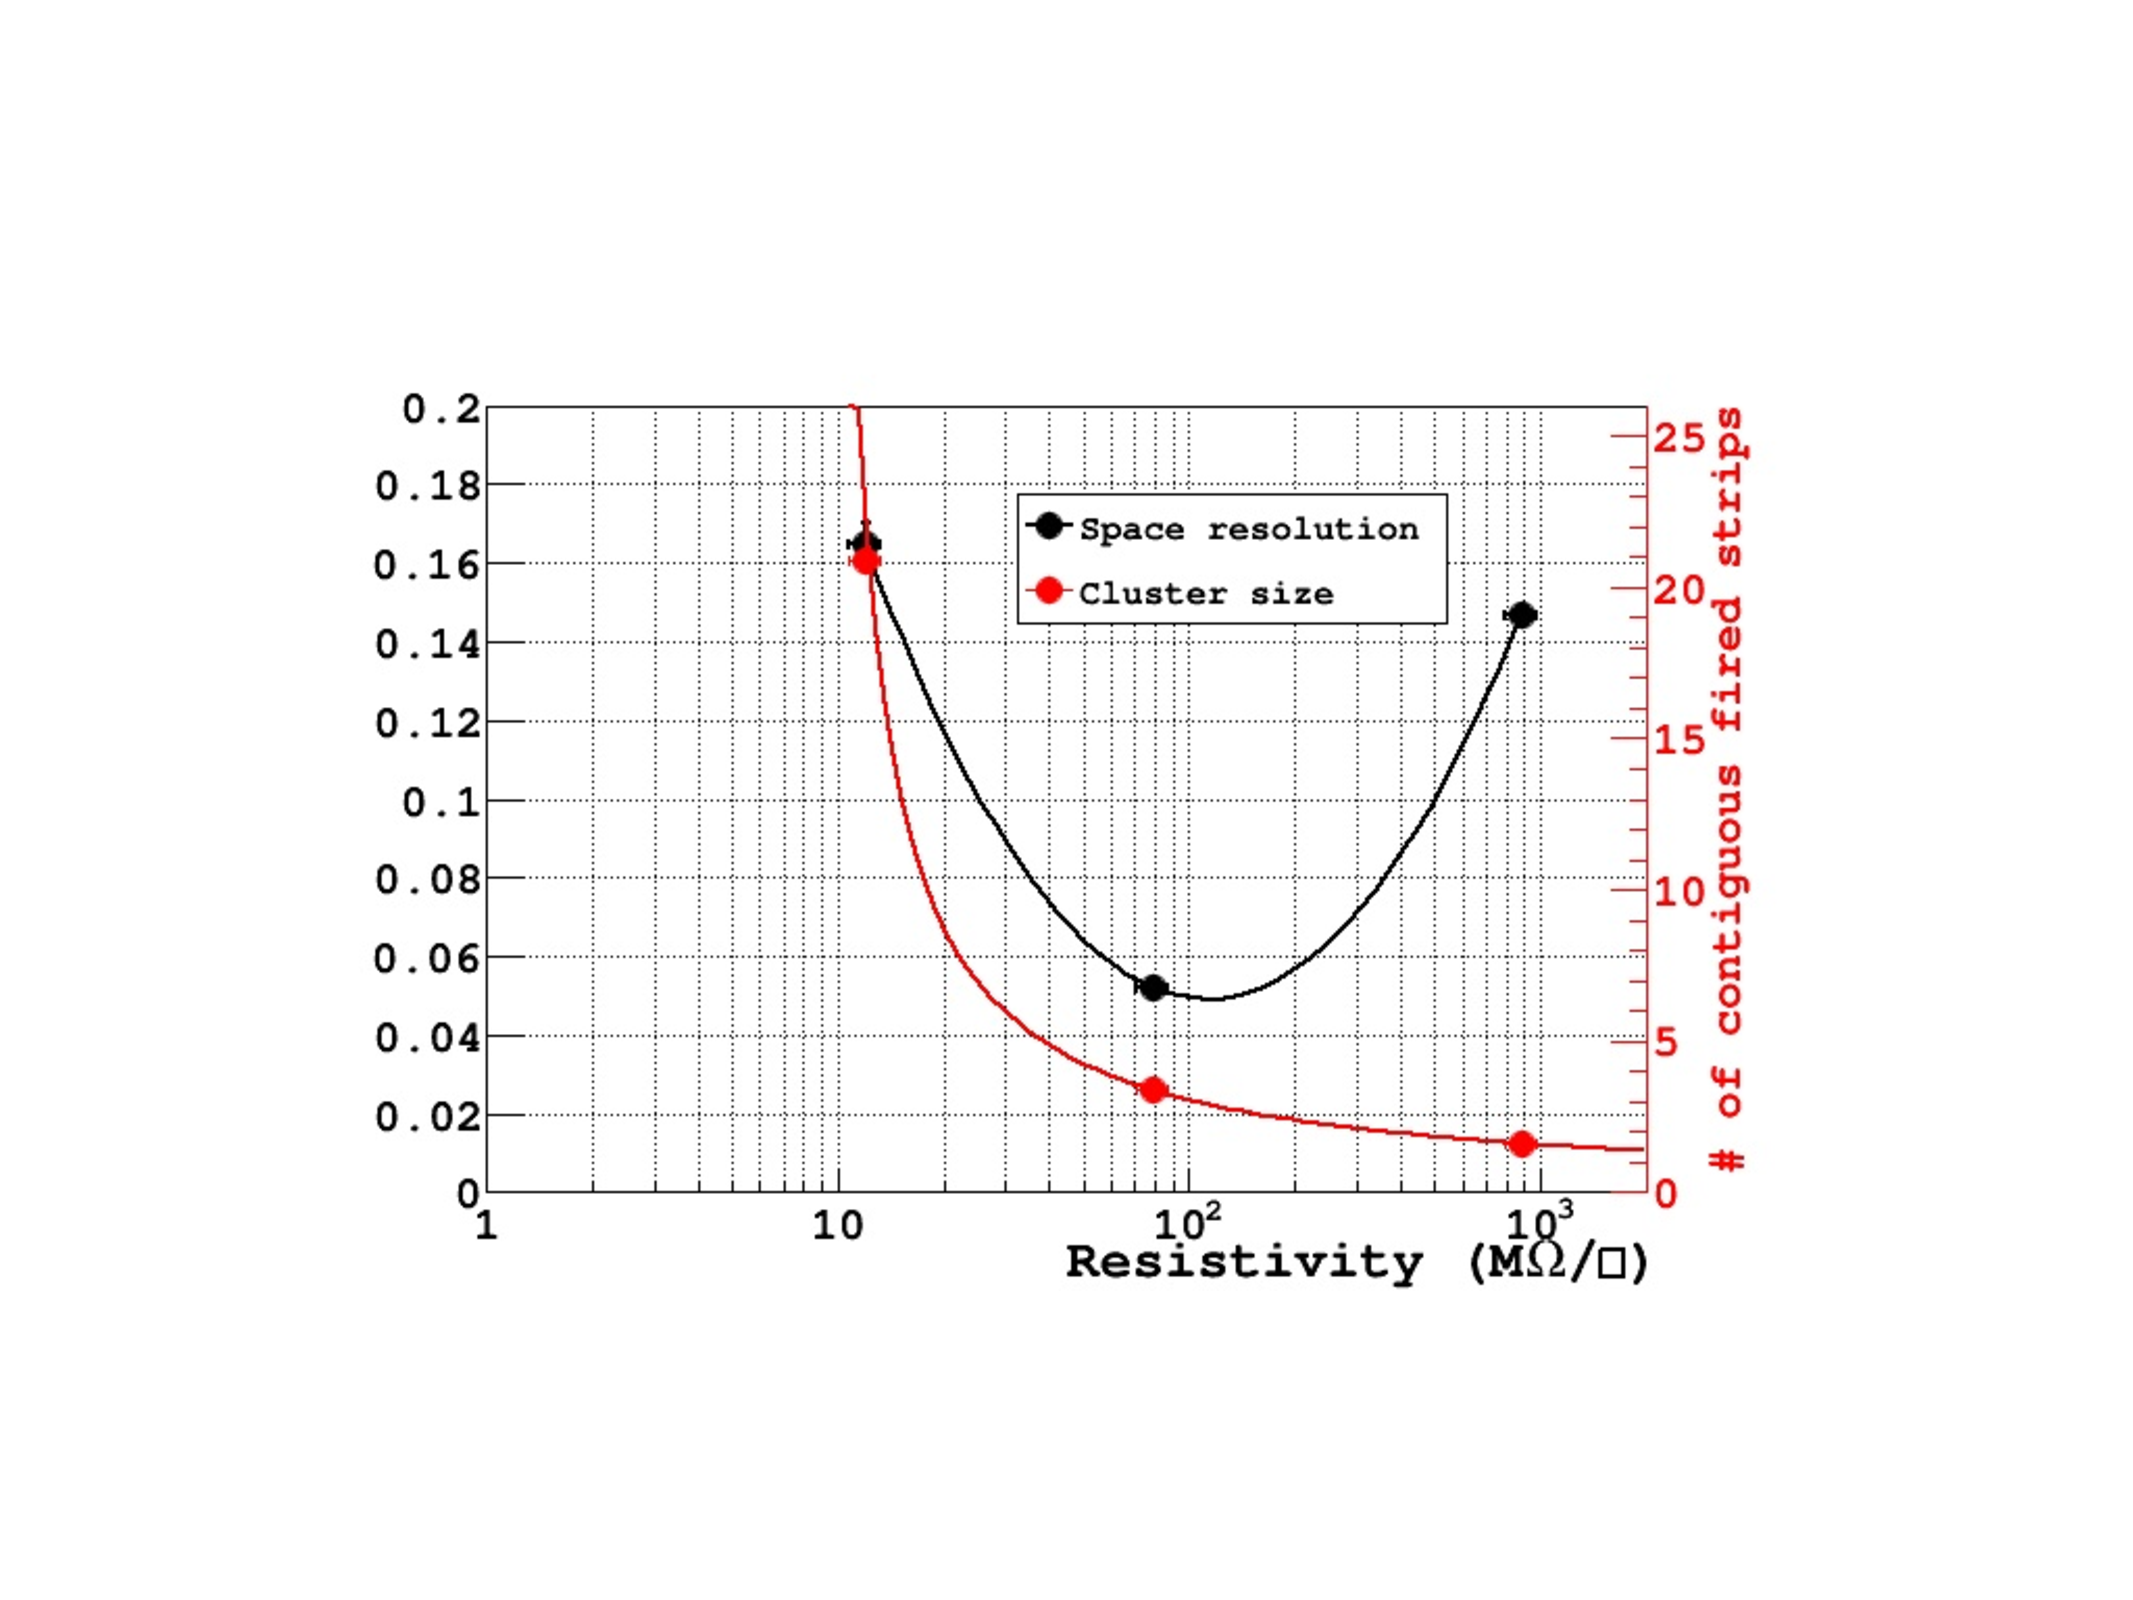
\includegraphics[scale=0.35]{Figures/Muon/microrwell-space-resolution_vs_rho.pdf}
        \caption{Space resolution and strip cluster size (0.4 mm strip pitch) as a function of the DLC resistivity.}
        \label{rho_res}
\end{figure}
%
%
\subsection{Large size $\mu$RWell detectors}
\label{sec:large-size}
%
Modern HEP experiments, as well as some specific applications of gaseous detectors, require for large area coverage. In particular the upgrade of the experiments at the HL-LHC at CERN needs to cover large regions with high precision rad-hard tracking devices.
%
\begin{figure}[h]
	\begin{center}
    	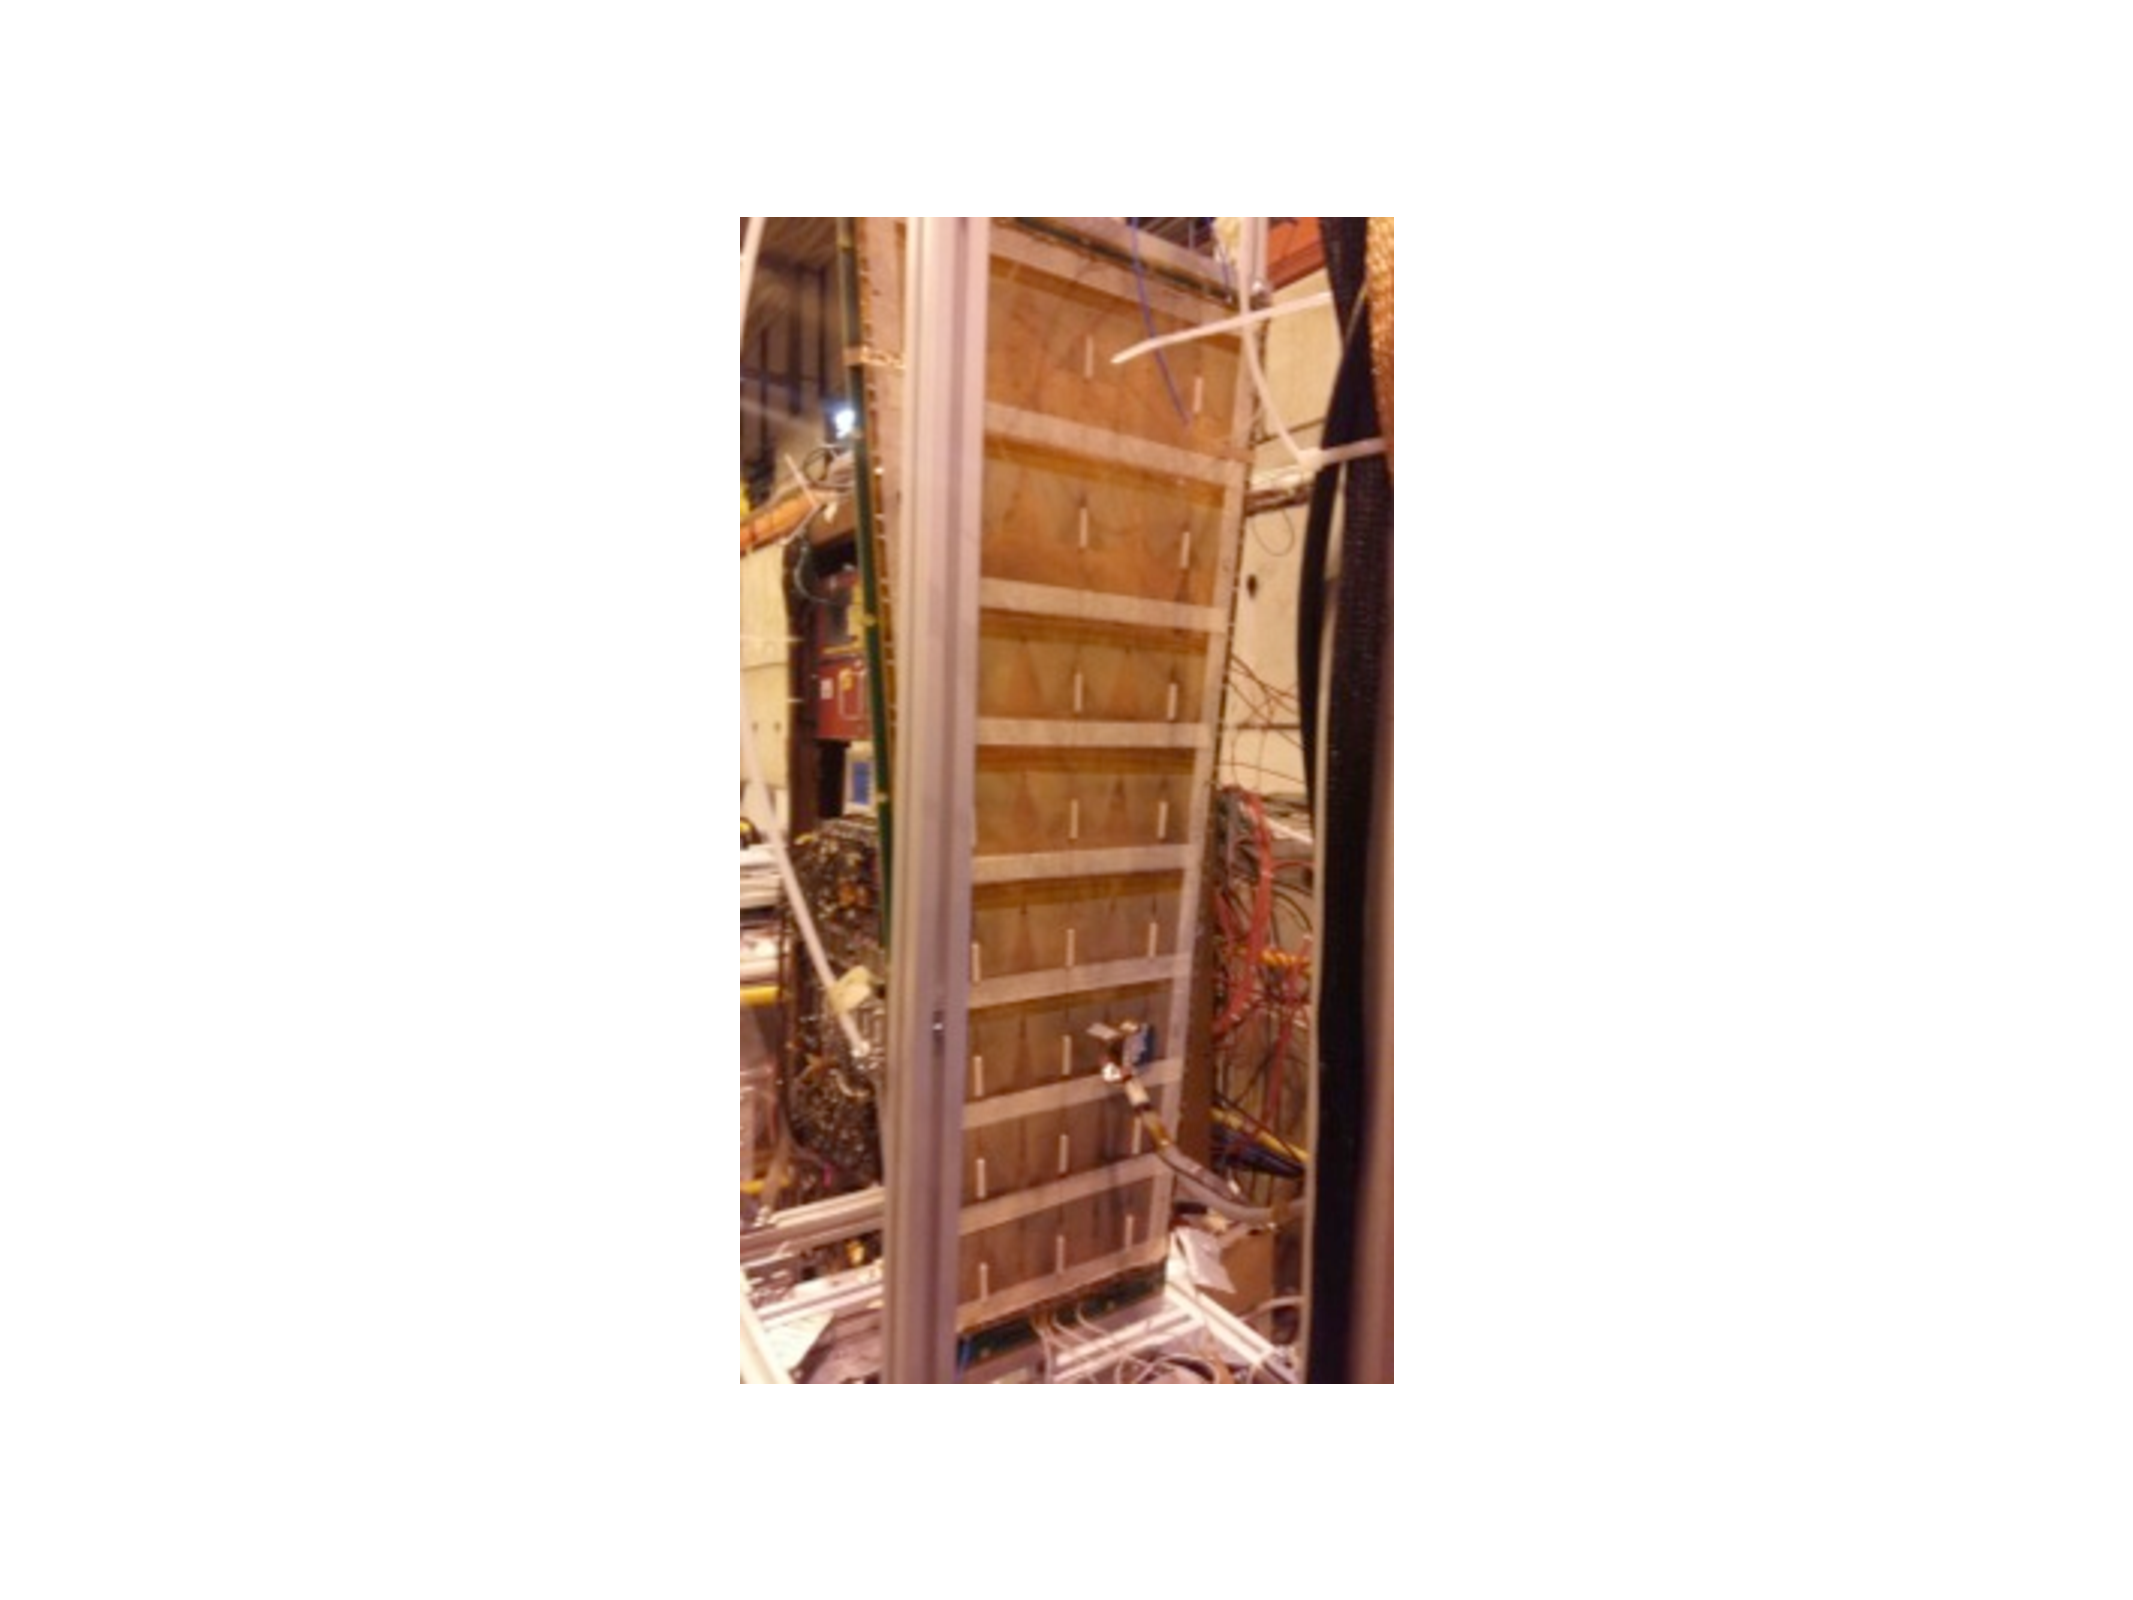
\includegraphics[scale=0.45]{Figures/Muon/microrwell-GE11.pdf}
        \caption{Picture of the GE1/1-$\mu$RWell prototype}
        \label{GE1/1}
    \end{center}
\end{figure}
%
The single-resistive layer $\mu$RWell is a mature technology to be proposed as tracking device for the CMS Phase2 upgrade of the muon detector. The upgrade in the end-cap region called GE2/1,  foresees several $\sim$2$\times$1 m$^2$ trapezoidal chambers to cover a global area of about 140 m$^2$. 
In this framework we have started an R\&D for the engineering, construction and test of large size single-resistive layer $\mu$RWells. The task has been accomplished in strict collaboration with an Italian PCB Company (ELTOS SpA, http://www.eltos.com/).\\
As a first step we have designed, built and characterized in a beam test at the H8-SPS area at CERN a $\sim$1.2$\times$0.5 m$^2$ $\mu$RWell (GE1/1-$\mu$RWell prototype), smaller than the final GE2/1, but $\sim$40 times larger than every $\mu$RWells prototype previously built (fig. \ref{GE1/1}). 
The results of the test will be discussed in section~\ref{section:uRWell-performance}.

\subsection{$\mu$RWell performances in test beams}
\label{section:uRWell-performance}

%Several of the results on $\mu$RWell prototypes presented in the following come from the R\&D work pursued by the CMS experiment at the LHC, within the framework of the Phase 2 upgrade of the forward Muon detector for the forthcoming High Luminosity phase of the LHC (HL-LHC) collider at CERN.
%These results are discussed here since this R\&D applies also to other future muon detectors with similar physics requirements.
%A large size $\mu$RWell prototype (GE11 size, roughly 0.5 m$^2$) was built and tested at the CERN H8 beam line during the 2016 test beam campaign with 150 GeV/c muons and pions. 
The GE1/1 prototype had a resistive DLC surface resistivity of about 70 M$\Omega\Box$ (in the \textit{low-rate} schema configuration). 
The strips pitch was 800 $\mu$m and the chamber was equipped with VFAT2 front-end electronics. 
The gas mixture used was Ar/CO$_2$/CF$_4$ (45/15/40), with a drift gap of 7 mm. 
Due to different used geometries for the amplification stage, the prototype was divided into two sectors (left and right) of slightly different gain. 
Both sectors were tested for efficiency and time resolution and the results compared with the performance of small $\mu$RWell prototypes (10 cm x 10cm, built in the \textit{high-rate} configuration) used into the same experimental setup and equipped with the same electronics. 
Figure~\ref{fig:urwell-eff-gain}a) shows the efficiency as a function of gain for the GE11 size prototype and two small (10x10 cm$^2$) $\mu$RWell prototypes: one can observe that the three detectors have an identical behavior. 
Figure~\ref{fig:urwell-eff-gain}b) shows the time resolution as a function of gain: a resolution better than 6 ns is obtained for all three $\mu$RWell prototypes for a gain of about 10000.

%
\begin{figure}[h!]
\centering
\begin{tabular}{cc}
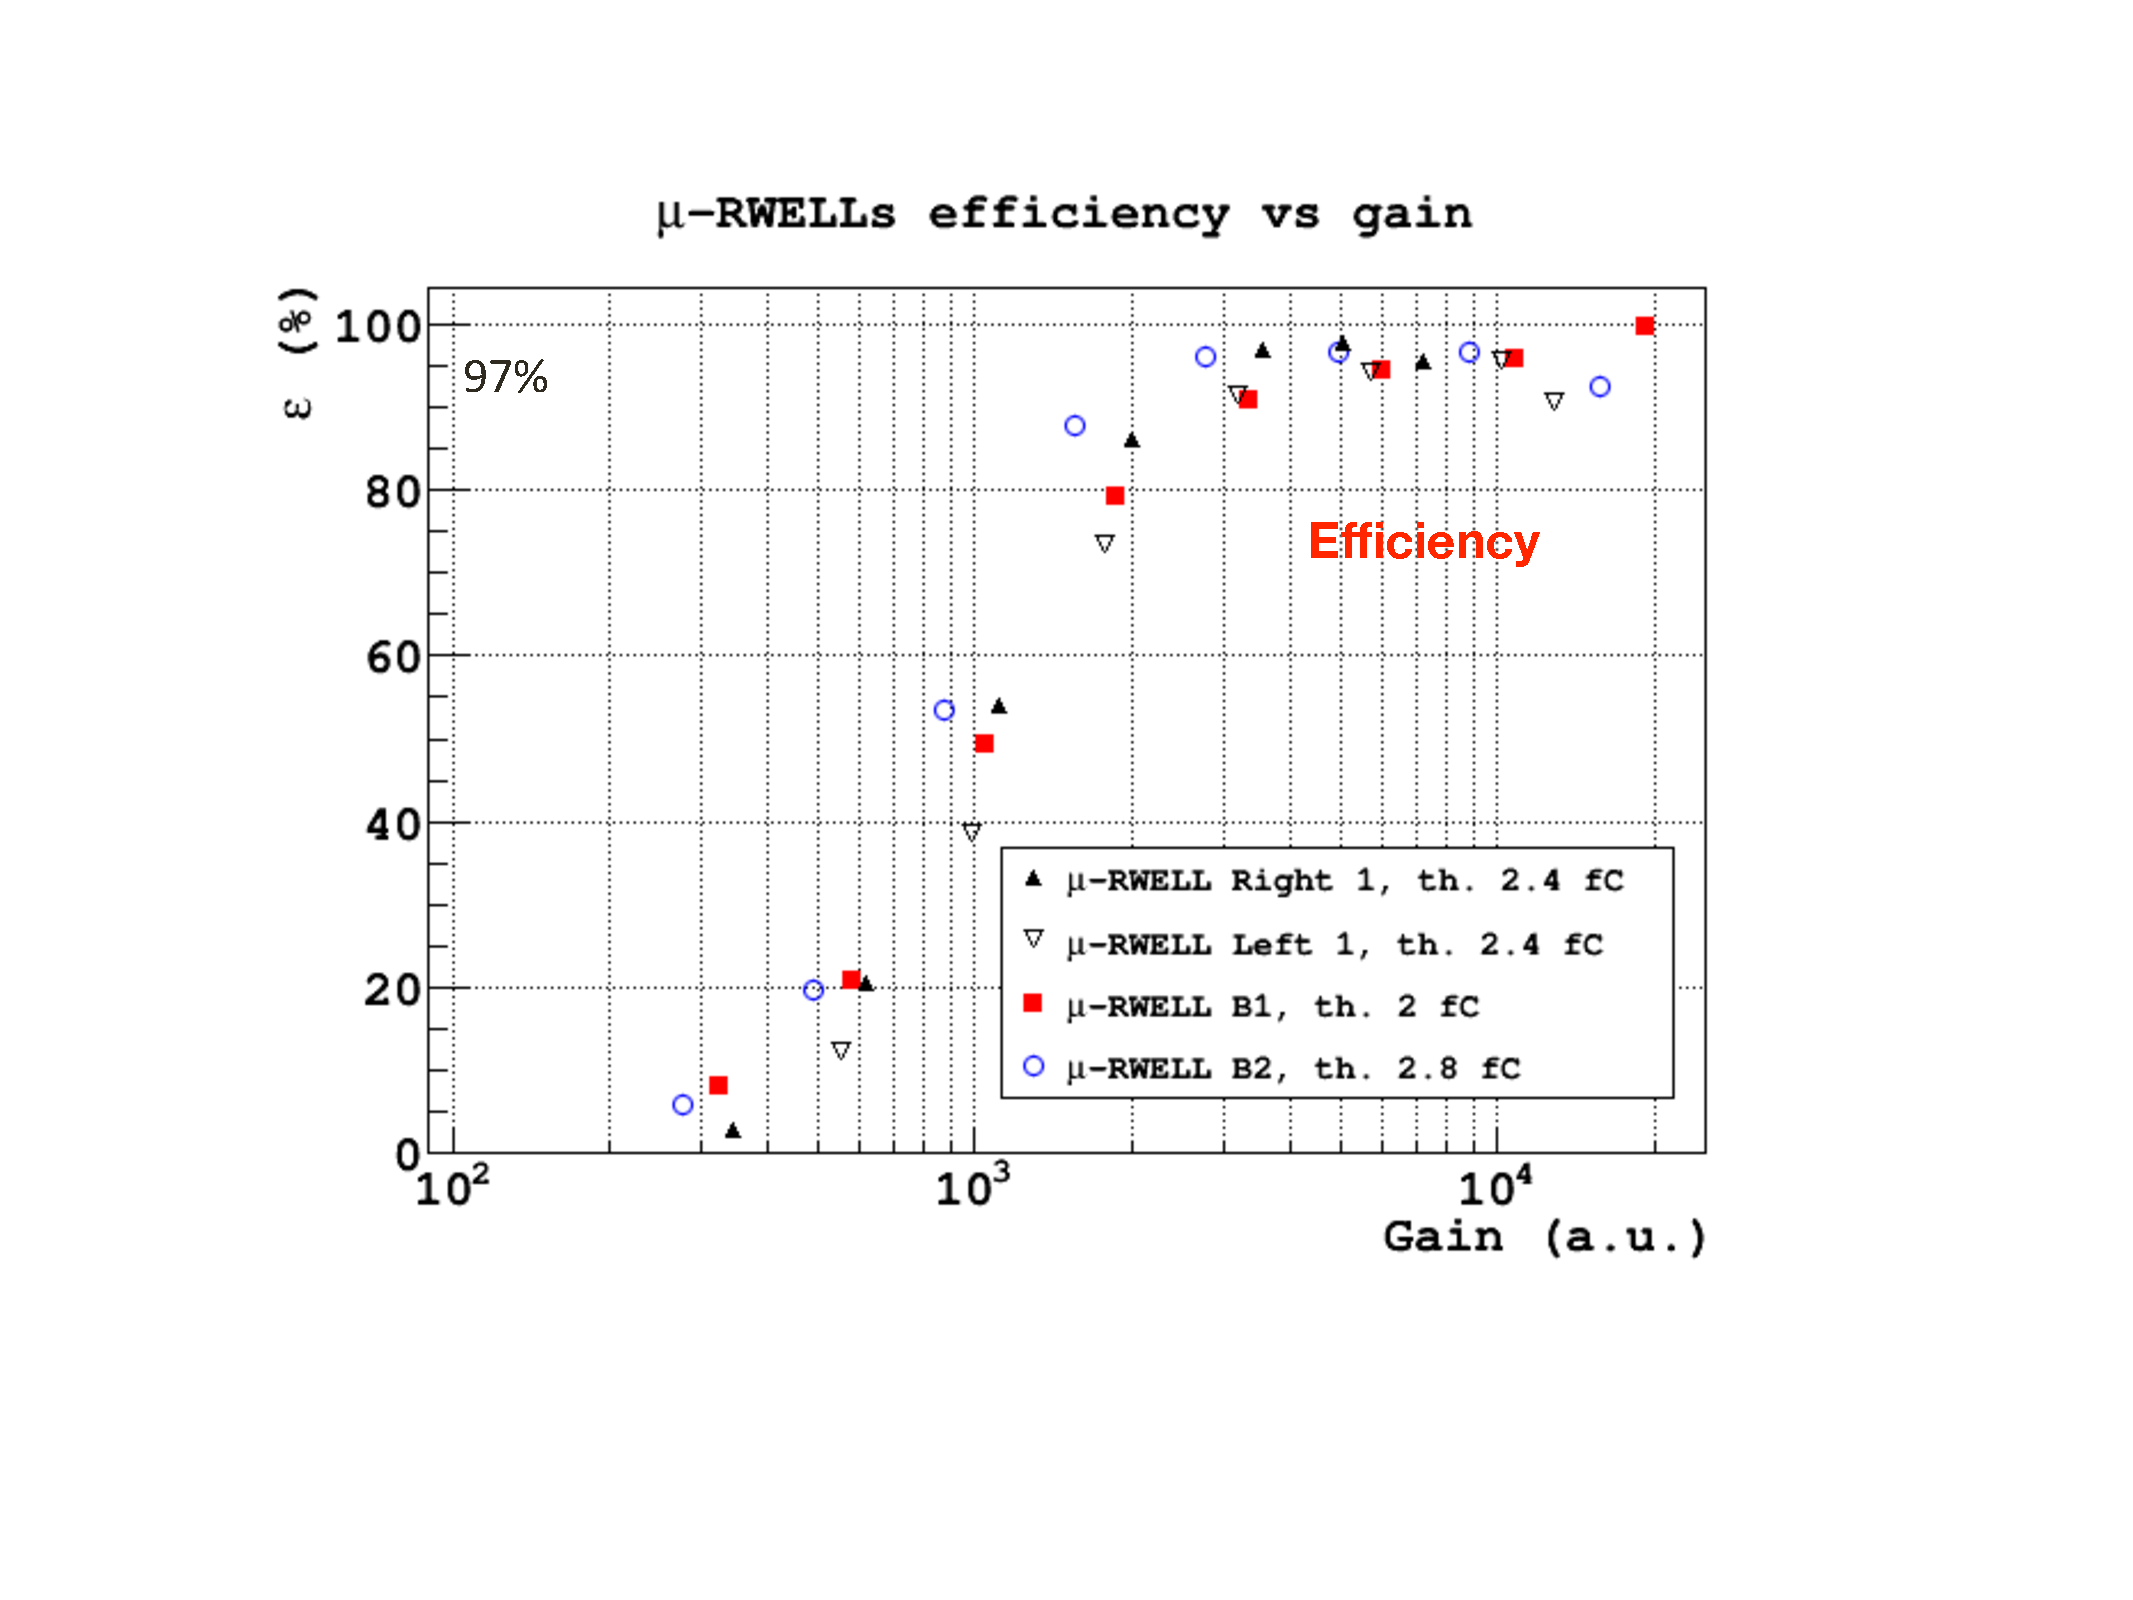
\includegraphics[width=0.5\textwidth]{Figures/Muon/microrwell-eff-gain.pdf} &
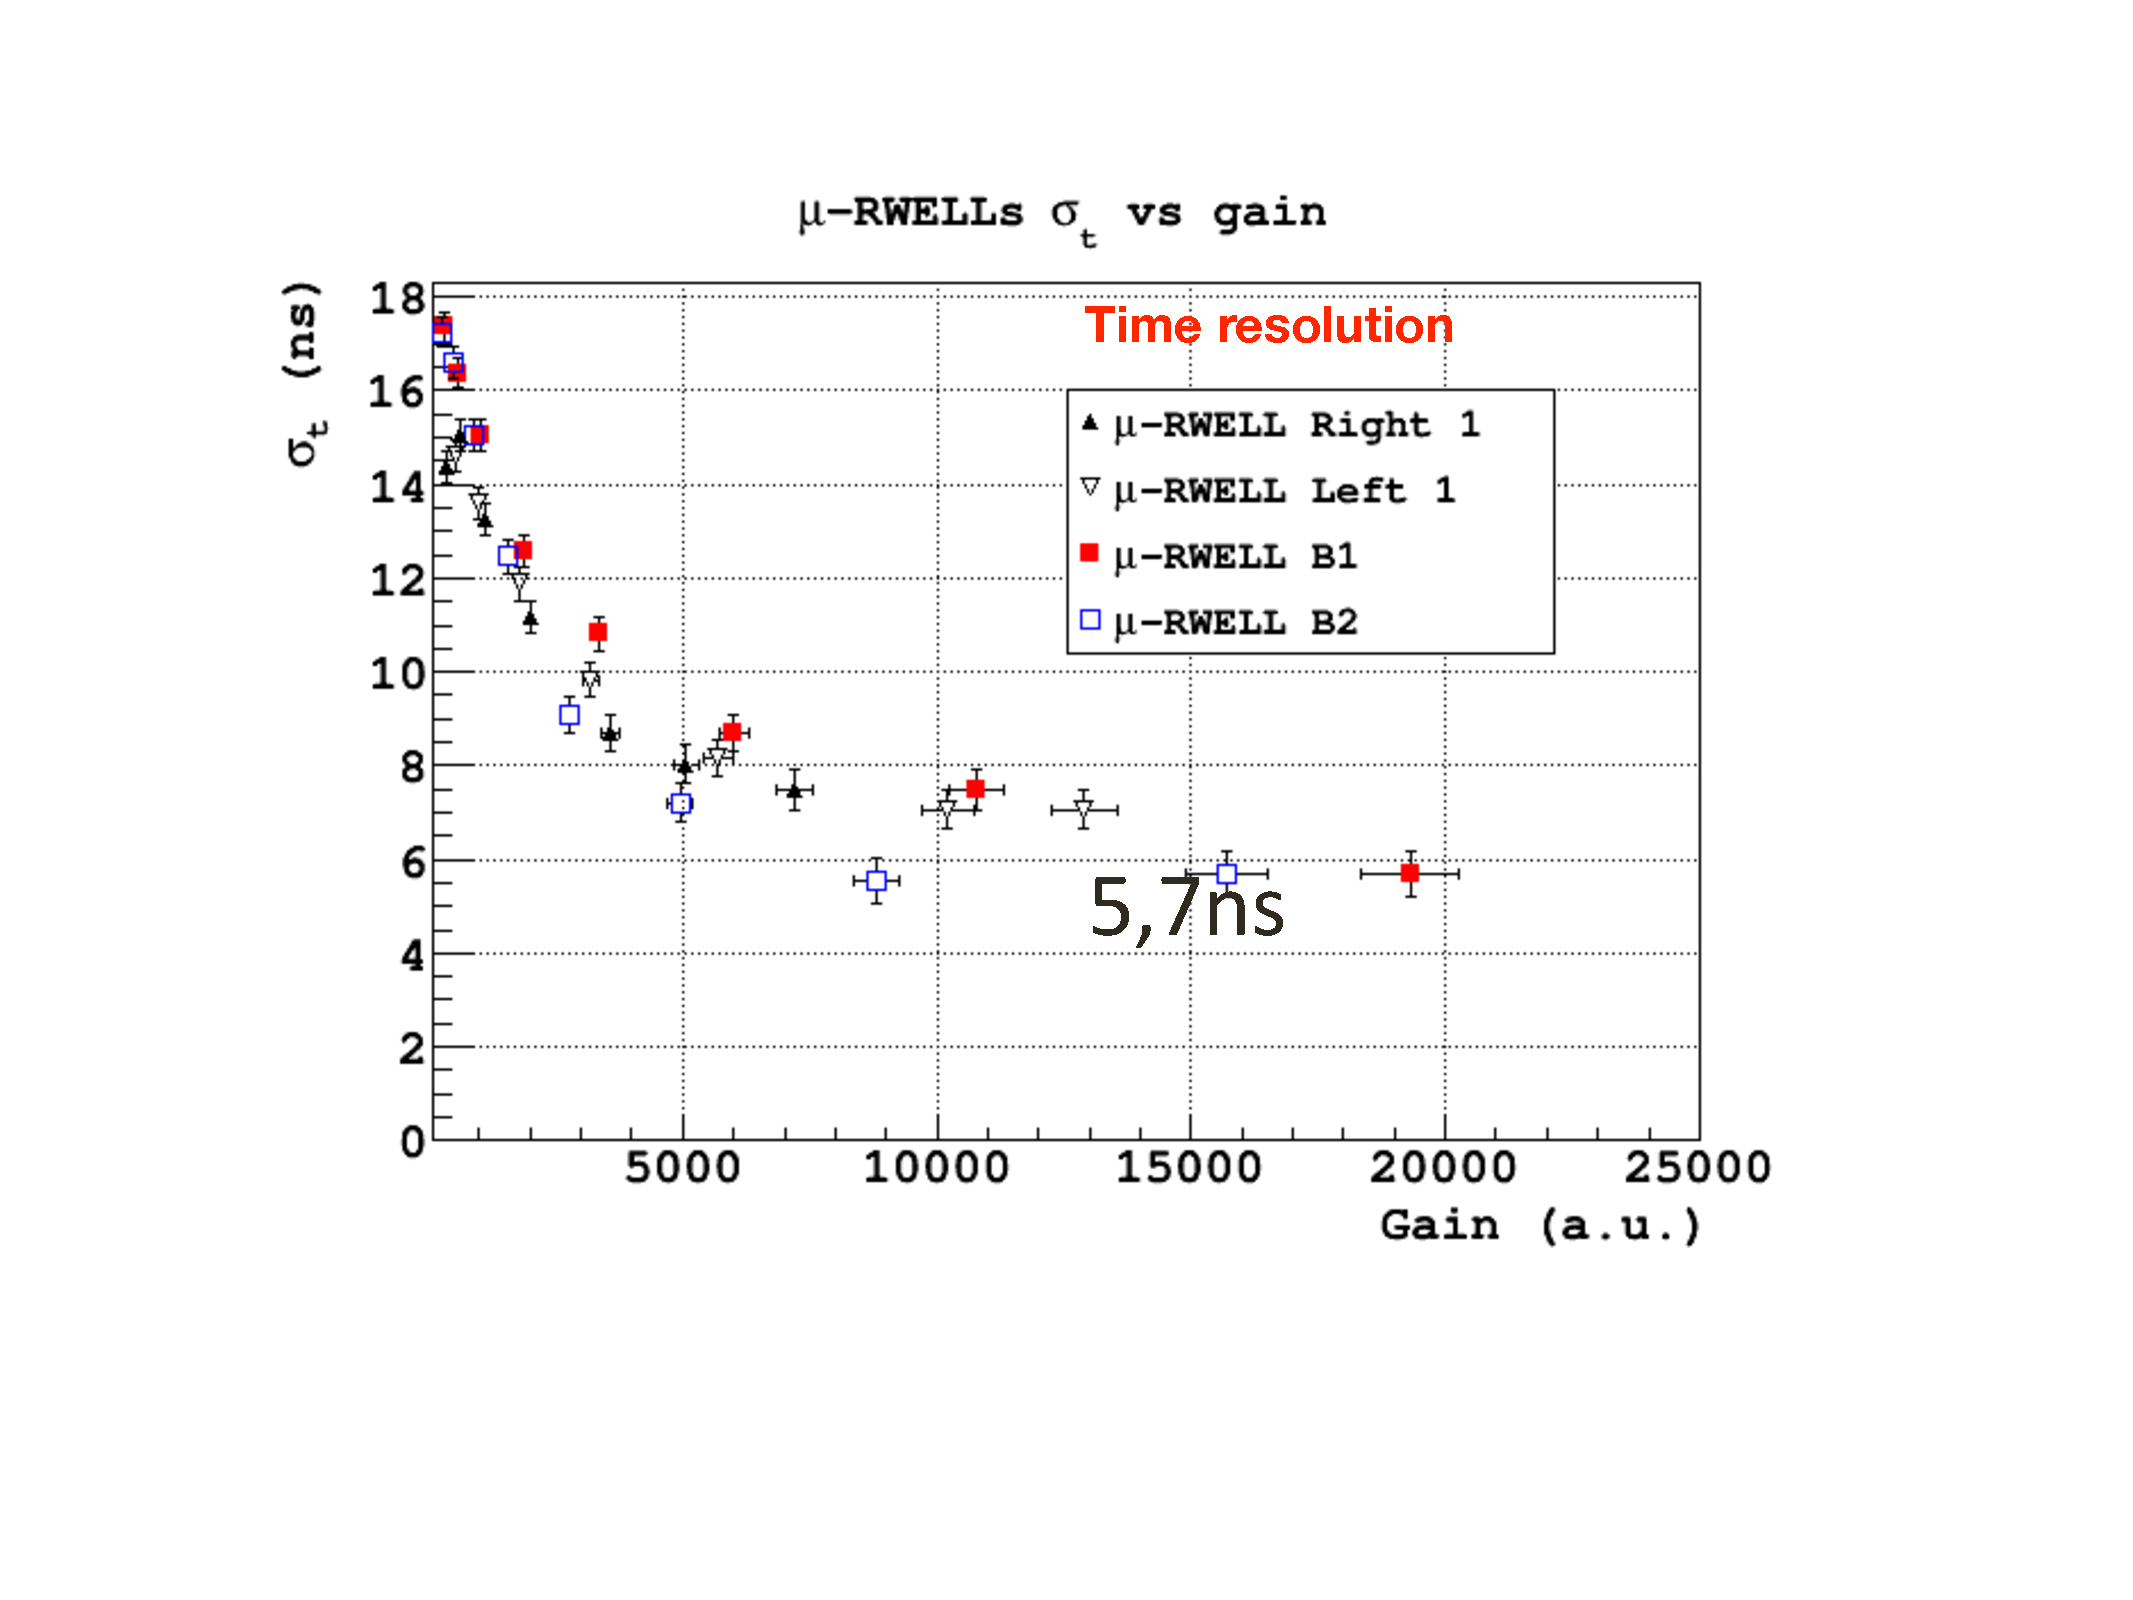
\includegraphics[width=0.5\textwidth]{Figures/Muon/microrwell-time-resolution-vs-gain.pdf} \\
\end{tabular}
\caption{a) Efficiency vs Gain. b) Time resolution vs Gain.}
\label{fig:urwell-eff-gain}
\end{figure}

In July 2017, the first GE21 20 degree sector equipped with two large area M4 $\mu$RWell detectors (each of dimensions ~50x60 cm$^2$) was assembled. It was subsequently exposed to a muon beam at the H4 test beam at CERN. The detector was placed on a remotely controllable moving platform in order to allow to scan the surface of the detector across the muon beam, as can be seen in figure 6. For the time being only one half of one M4 could be equipped with readout electronics and horizontal scans across one half of the M4 at the time were performed. The GE21 sector was flushed with an ARCO$_2$ 70-30 gas mixture. The beam line was equipped with a tracker composed of two GEM detectors and two small size $\mu$RWell prototypes. The efficiency of the GE21 sector was defined as the number of triple coincidences GE21xGEM1xGEM2 divided by the double coincidence GEM1xGEM2.
In figure~\ref{fig:GE2/1} a picture of the GE21 sector equipped with two large are M4 detectors is shown in the H4 beam line at CERN.

%
\begin{figure}[h]
	\begin{center}
    	\includegraphics[scale=0.45]{Figures/Muon/microrwell-GE21.pdf}
        \caption{Picture of the GE2/1 sector with two M4 $\mu$RWell prototypes}
        \label{GE2/1}
    \end{center}
\end{figure}

Figure~\ref{fig:urwell-GE21-eff-gain} shows the results obtained for the GE21 efficiency as function of the HV applied to its amplification stage. 
One can observe the very regular curve and the plateau is reached at approximately 520V.
As operating voltage 530 V was chosen, that is in the middle of the HV plateau. The nominal gain at this operating voltage is about 10000. Two horizontals scans were then performed at this voltage across the whole surface of one M4 detector: the two scans were performed at two vertical positions separated by 20 cm in height, in order to illuminate the whole surface of the detector.
Figure~\ref{fig:urwell-GE21-uniformity} shows the efficiency obtained in the various points of the two horizontal scans. 
Apart from the points at the edge of the M4 detector where the muon beam in not anymore completely contained in the M4 surface, all other points are within 98-99\% efficiency, therefore showing the excellent uniformity achieved by the detector over all its surface. 
This is also nicely visible in figure~\ref{fig:urwell-GE21-uniformity-2D}, where the trapezoidal shape of the detector is drawn on top of the 2D plot.

%
\begin{figure}[h!]
\centering
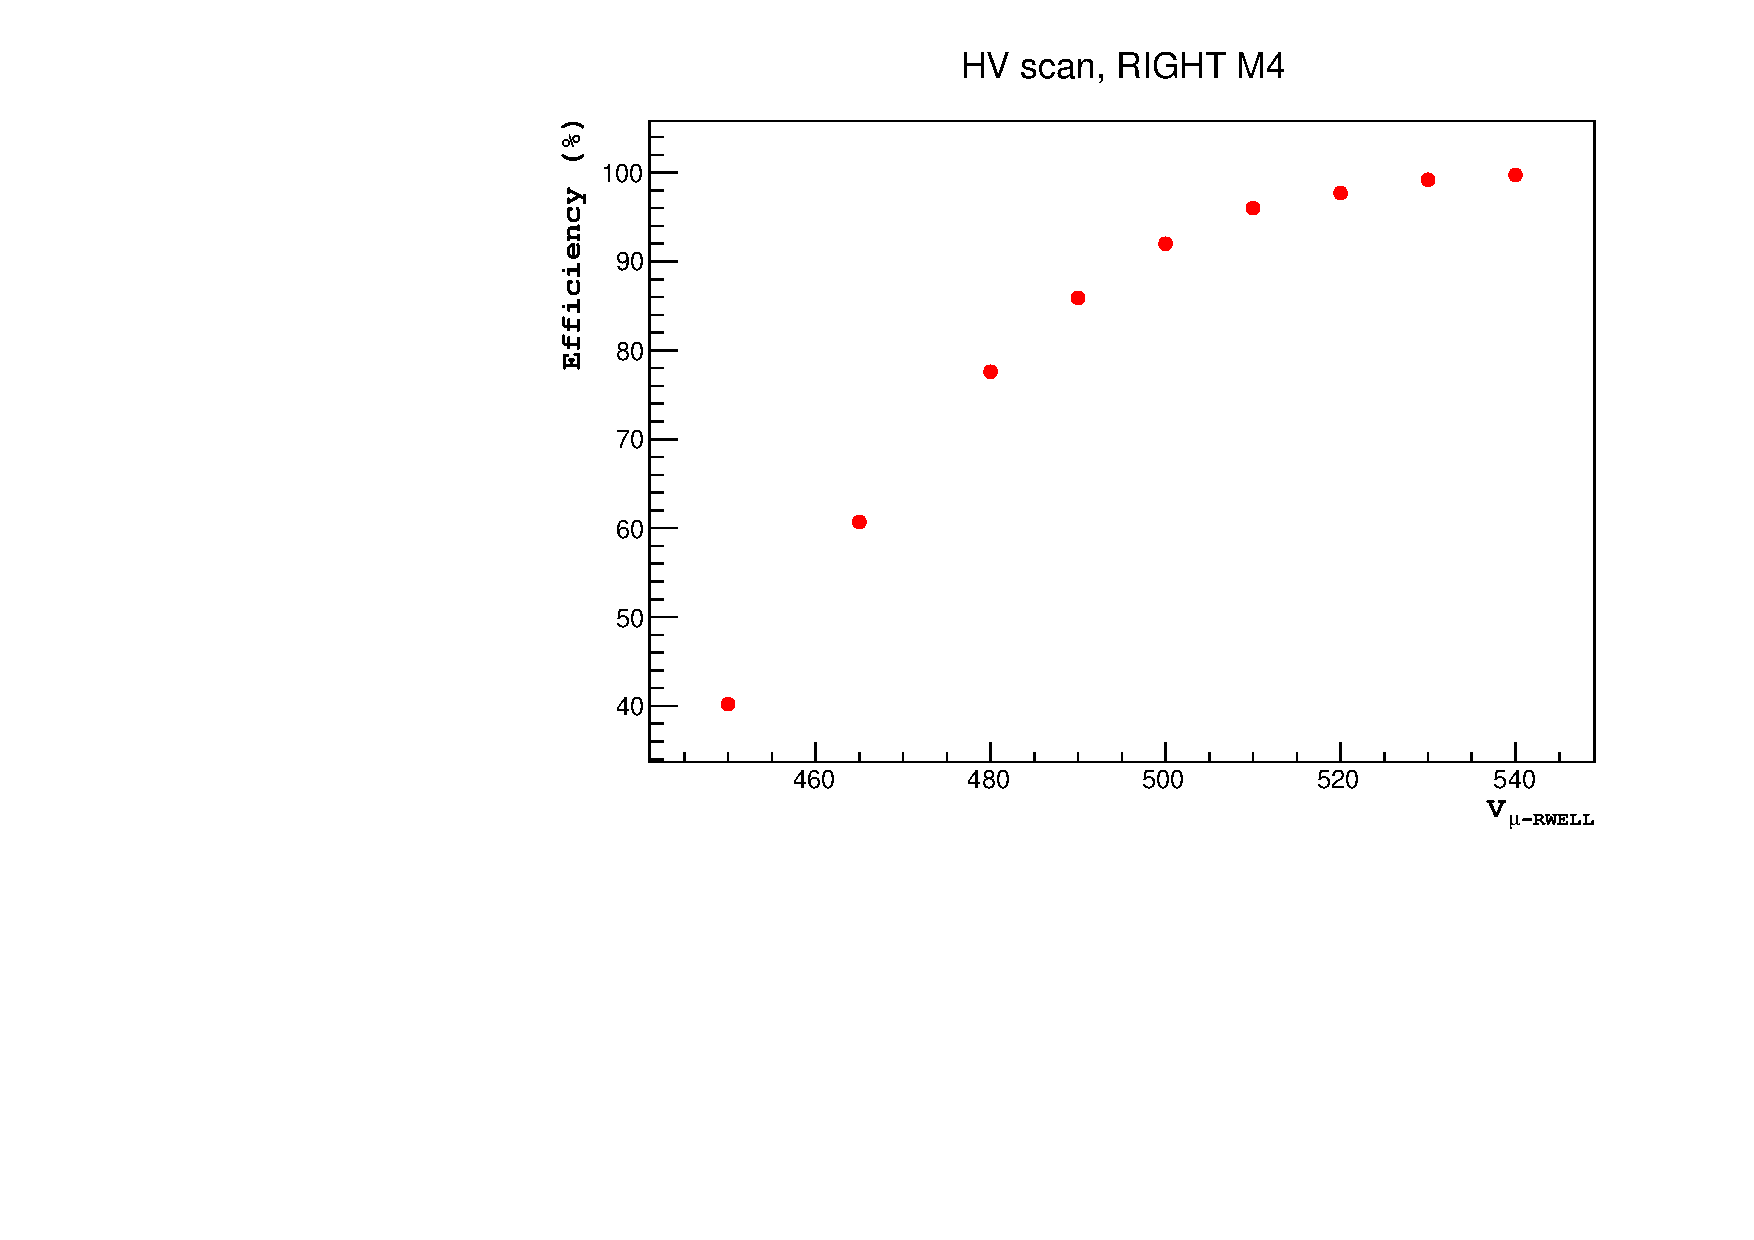
\includegraphics[width=0.5\textwidth]{Figures/Muon/microrwell-GE21-eff-gain.pdf}
\caption{GE21 efficiency as a function of the HV applied to the amplification kapton foil. The plateau is reached at about 520 V.}
\label{fig:urwell-GE21-eff-gain}
\end{figure}

%
\begin{figure}[h!]
\centering
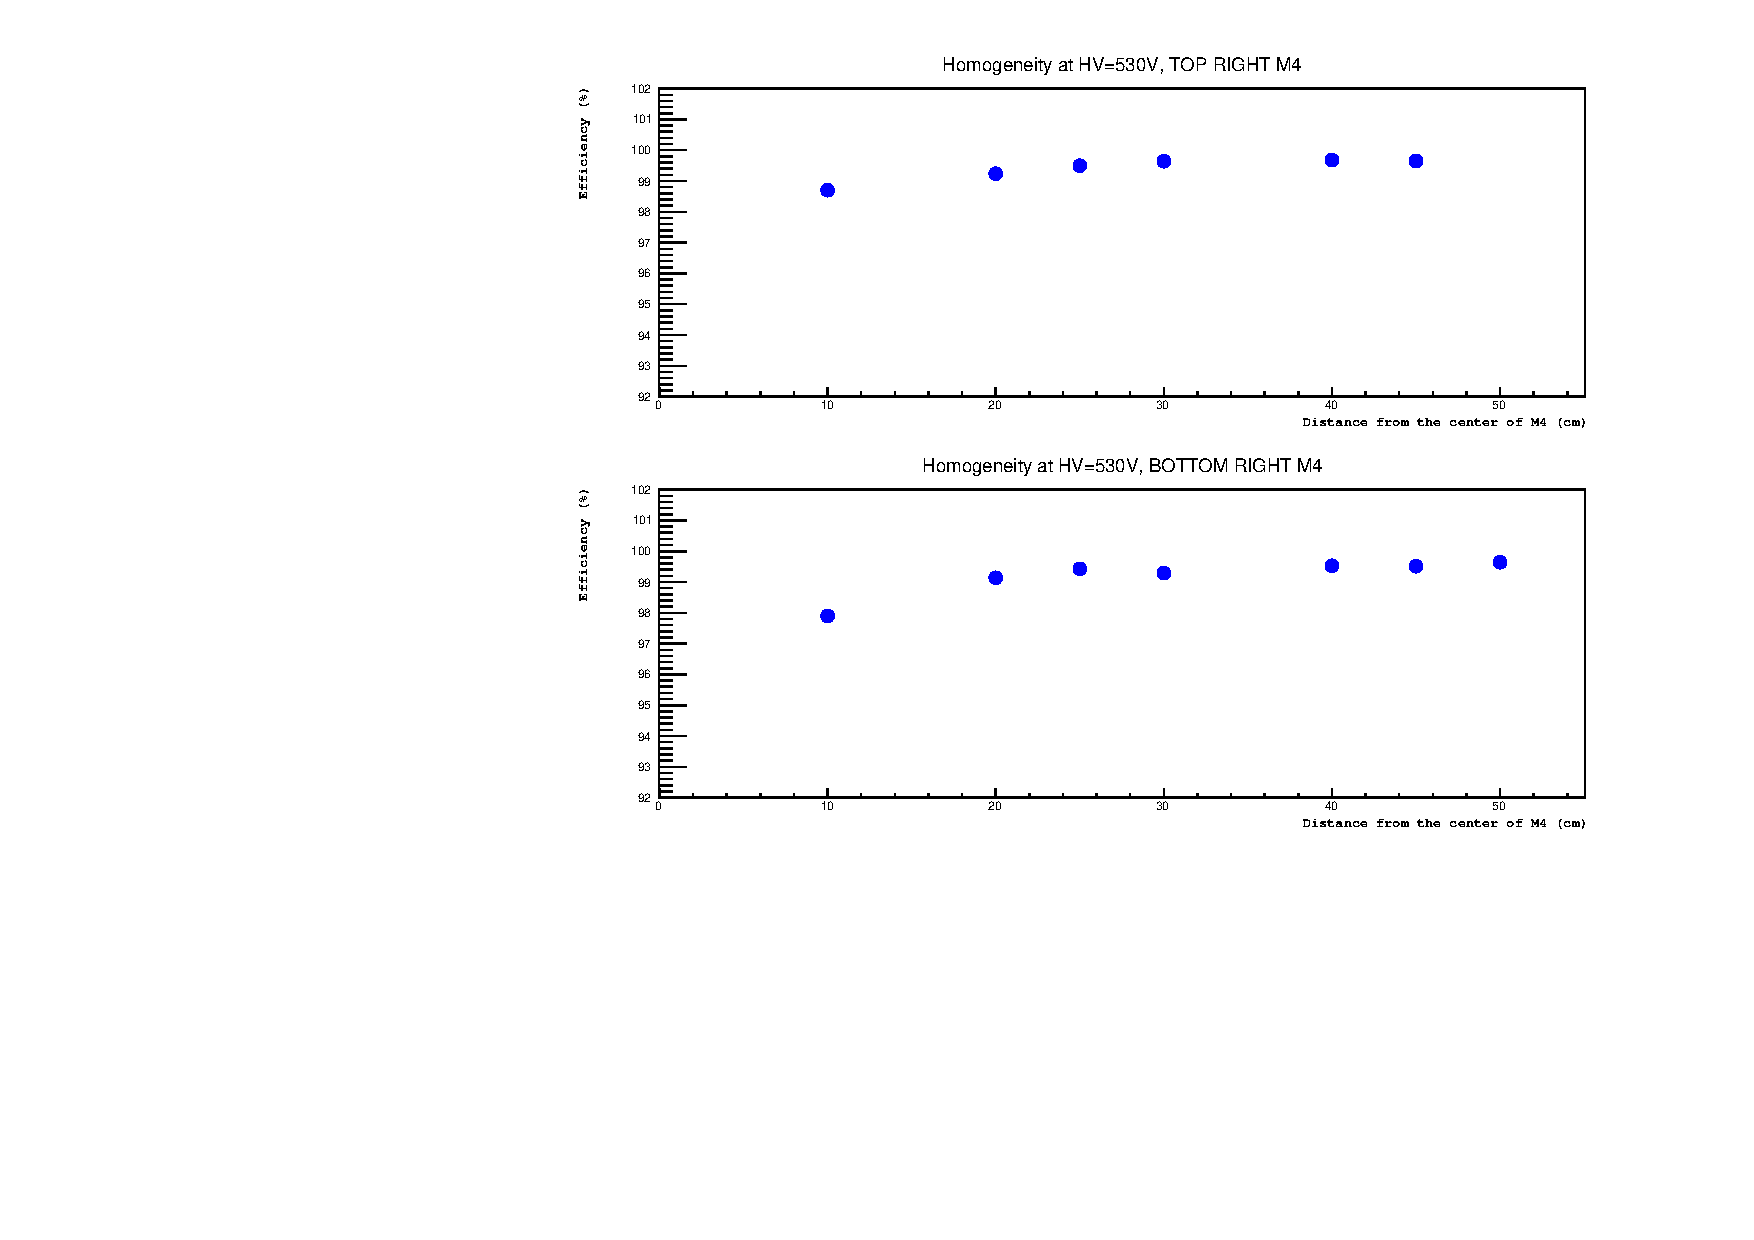
\includegraphics[width=0.7\textwidth]{Figures/Muon/microrwell-GE21-uniformity.pdf}
\caption{GE21 efficiency across the whole surface of one M4 detector. Two horizontal scans were performed in two vertical positions separated by 20 cm in height. The points at lower efficiency are obtained when the muon beam is not completely contained in the surface of the M4 detector. All other points are within 98-99\% efficiency providing an excellent uniformity.}
\label{fig:urwell-GE21-uniformity}
\end{figure}

%
\begin{figure}[h!]
\centering
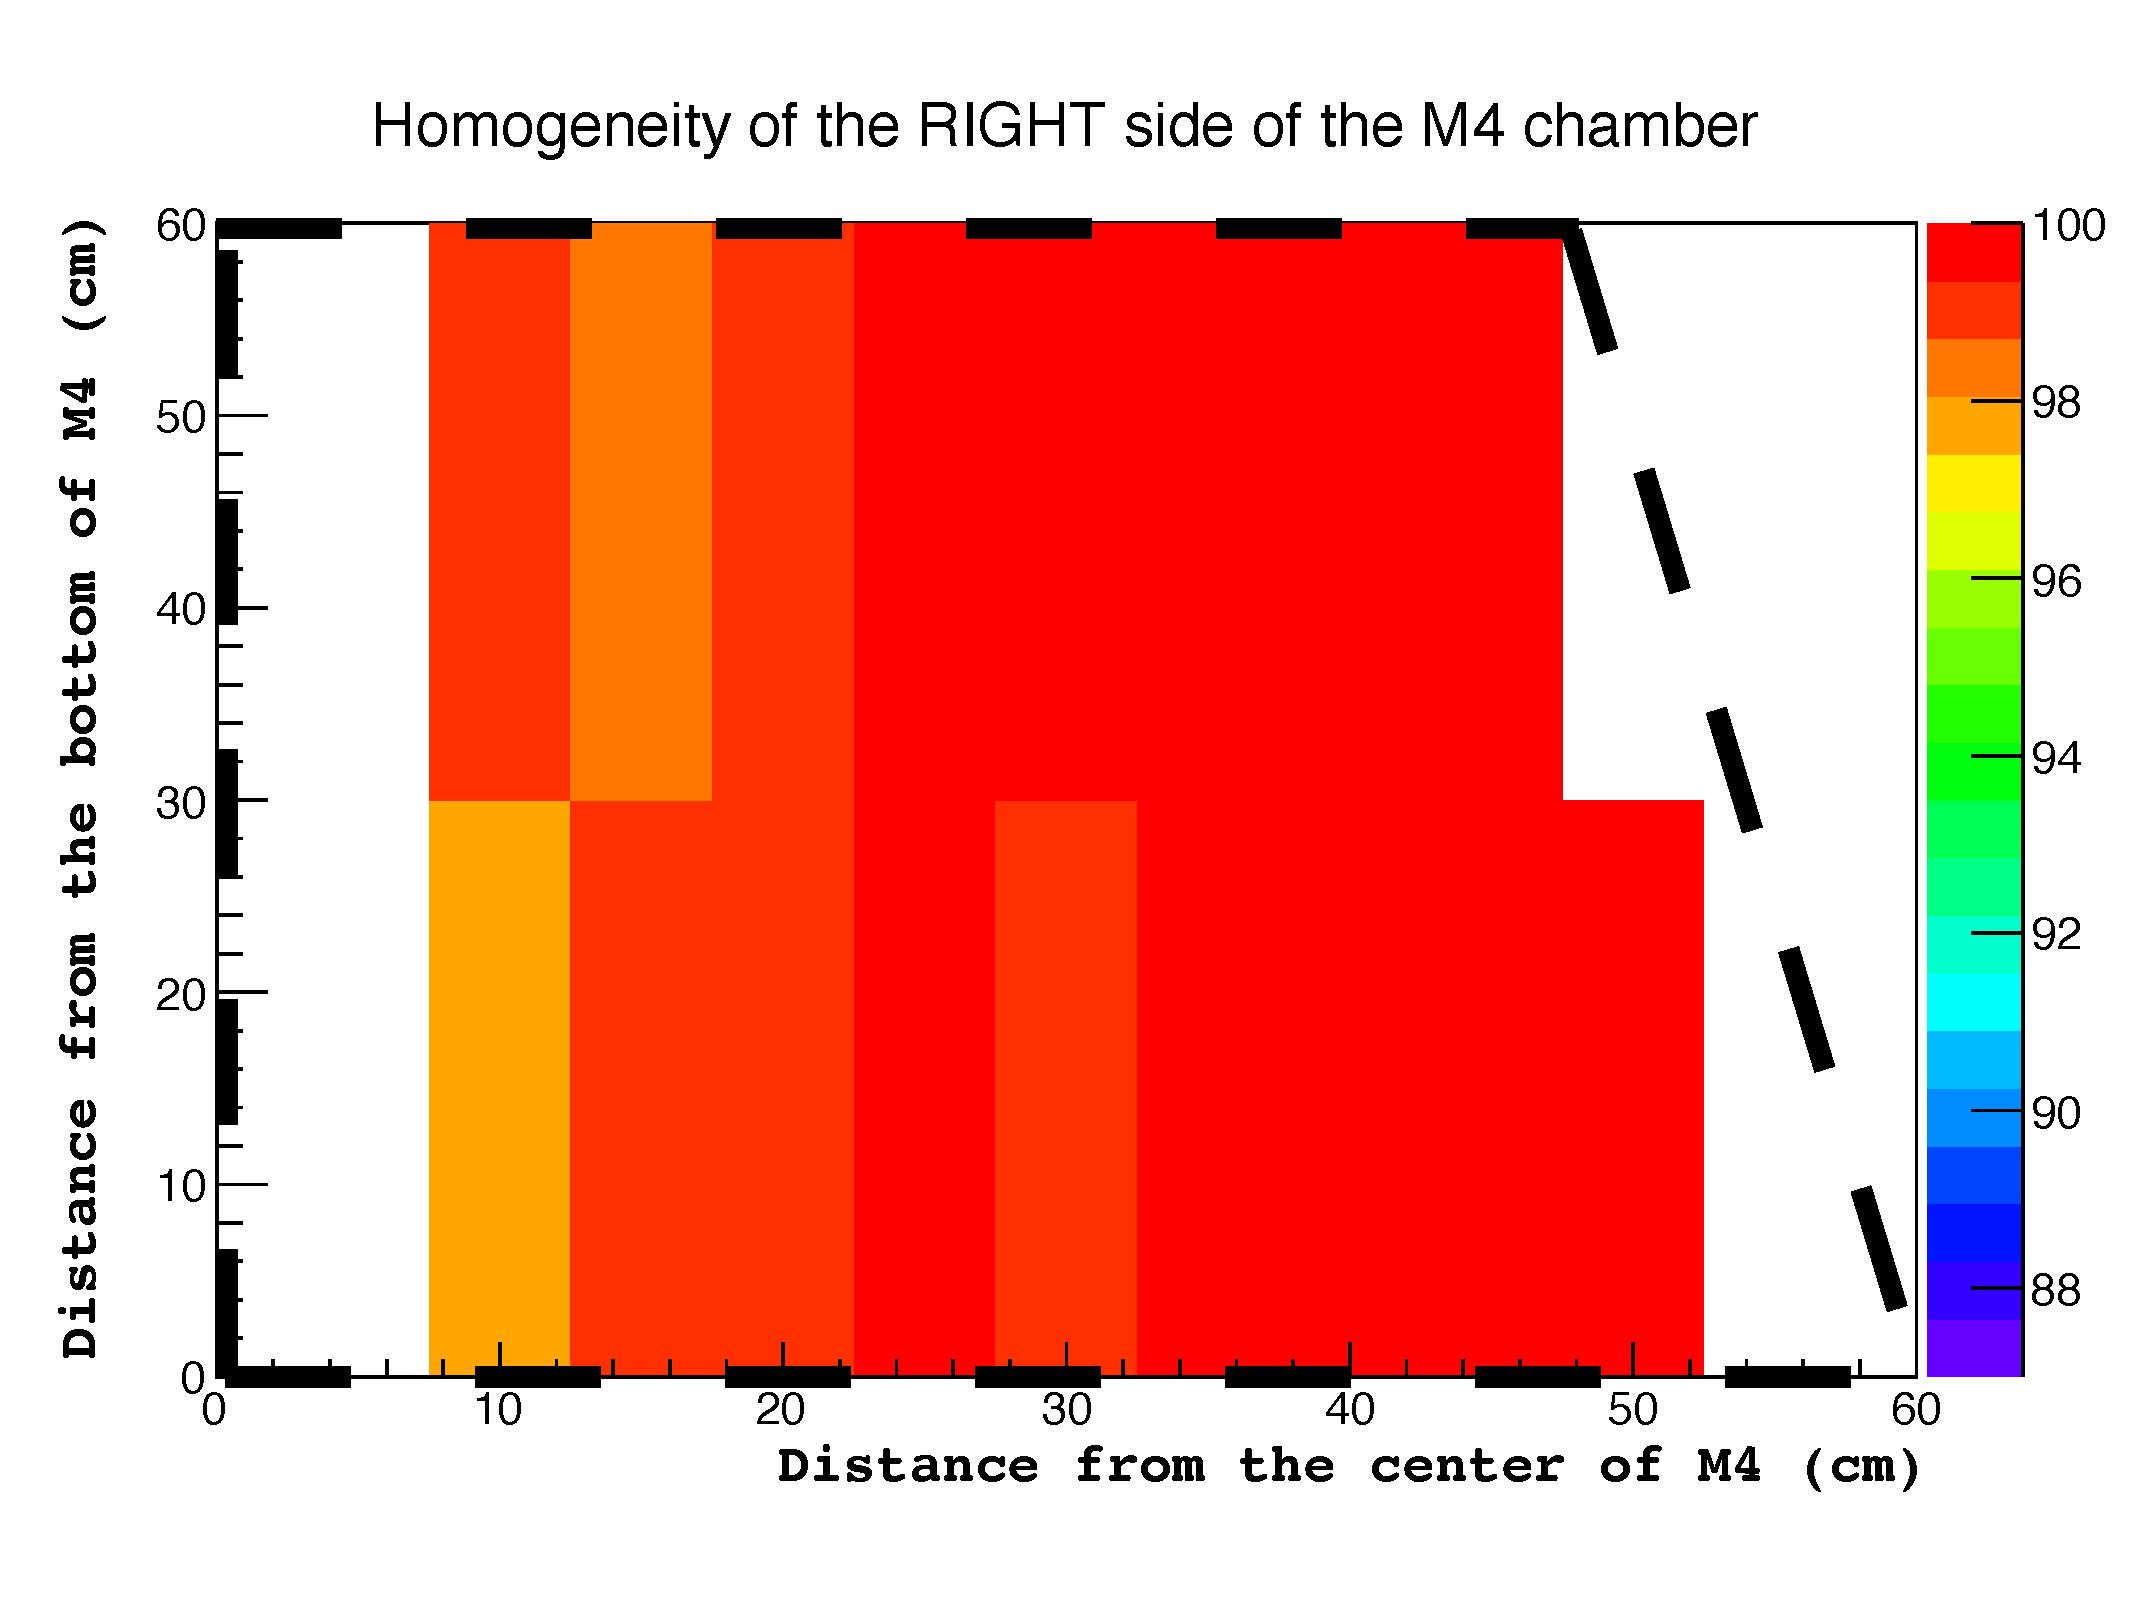
\includegraphics[width=0.7\textwidth]{Figures/Muon/microrwell-GE21-uniformity-2D.pdf}
\caption{M4 2D plot of efficiency across the whole surface. The trapezoidal shape of the detector is drawn on top of the plot.}
\label{fig:urwell-GE21-uniformity-2D}
\end{figure}



\subsubsection{MicroRWell ageing tests at the GIF++}
\label{section:uRWell-ageing}

From April 2017, the GE11 size $\mu$RWell prototype has been exposed to the GIF++ high-intensity source, together with two smaller prototypes. 
This has been done to verify the behavior of the $\mu$RWell technology under high irradiation, equivalent to several years of running at the HL-LHC in the GE2/1 environment. 
The GE11 size detector is since then operated with an ArCO$_2$ 70-30 gas mixture.
At the end of August 2017, the detector has already accumulated a dose equivalent to ~23 mC/cm$^2$, as can be seen in figure~\ref{fig:urwell-int-dose} , that corresponds to more than 100 years of operation under HL-LHC conditions.

%

\begin{figure}[h!]
\centering
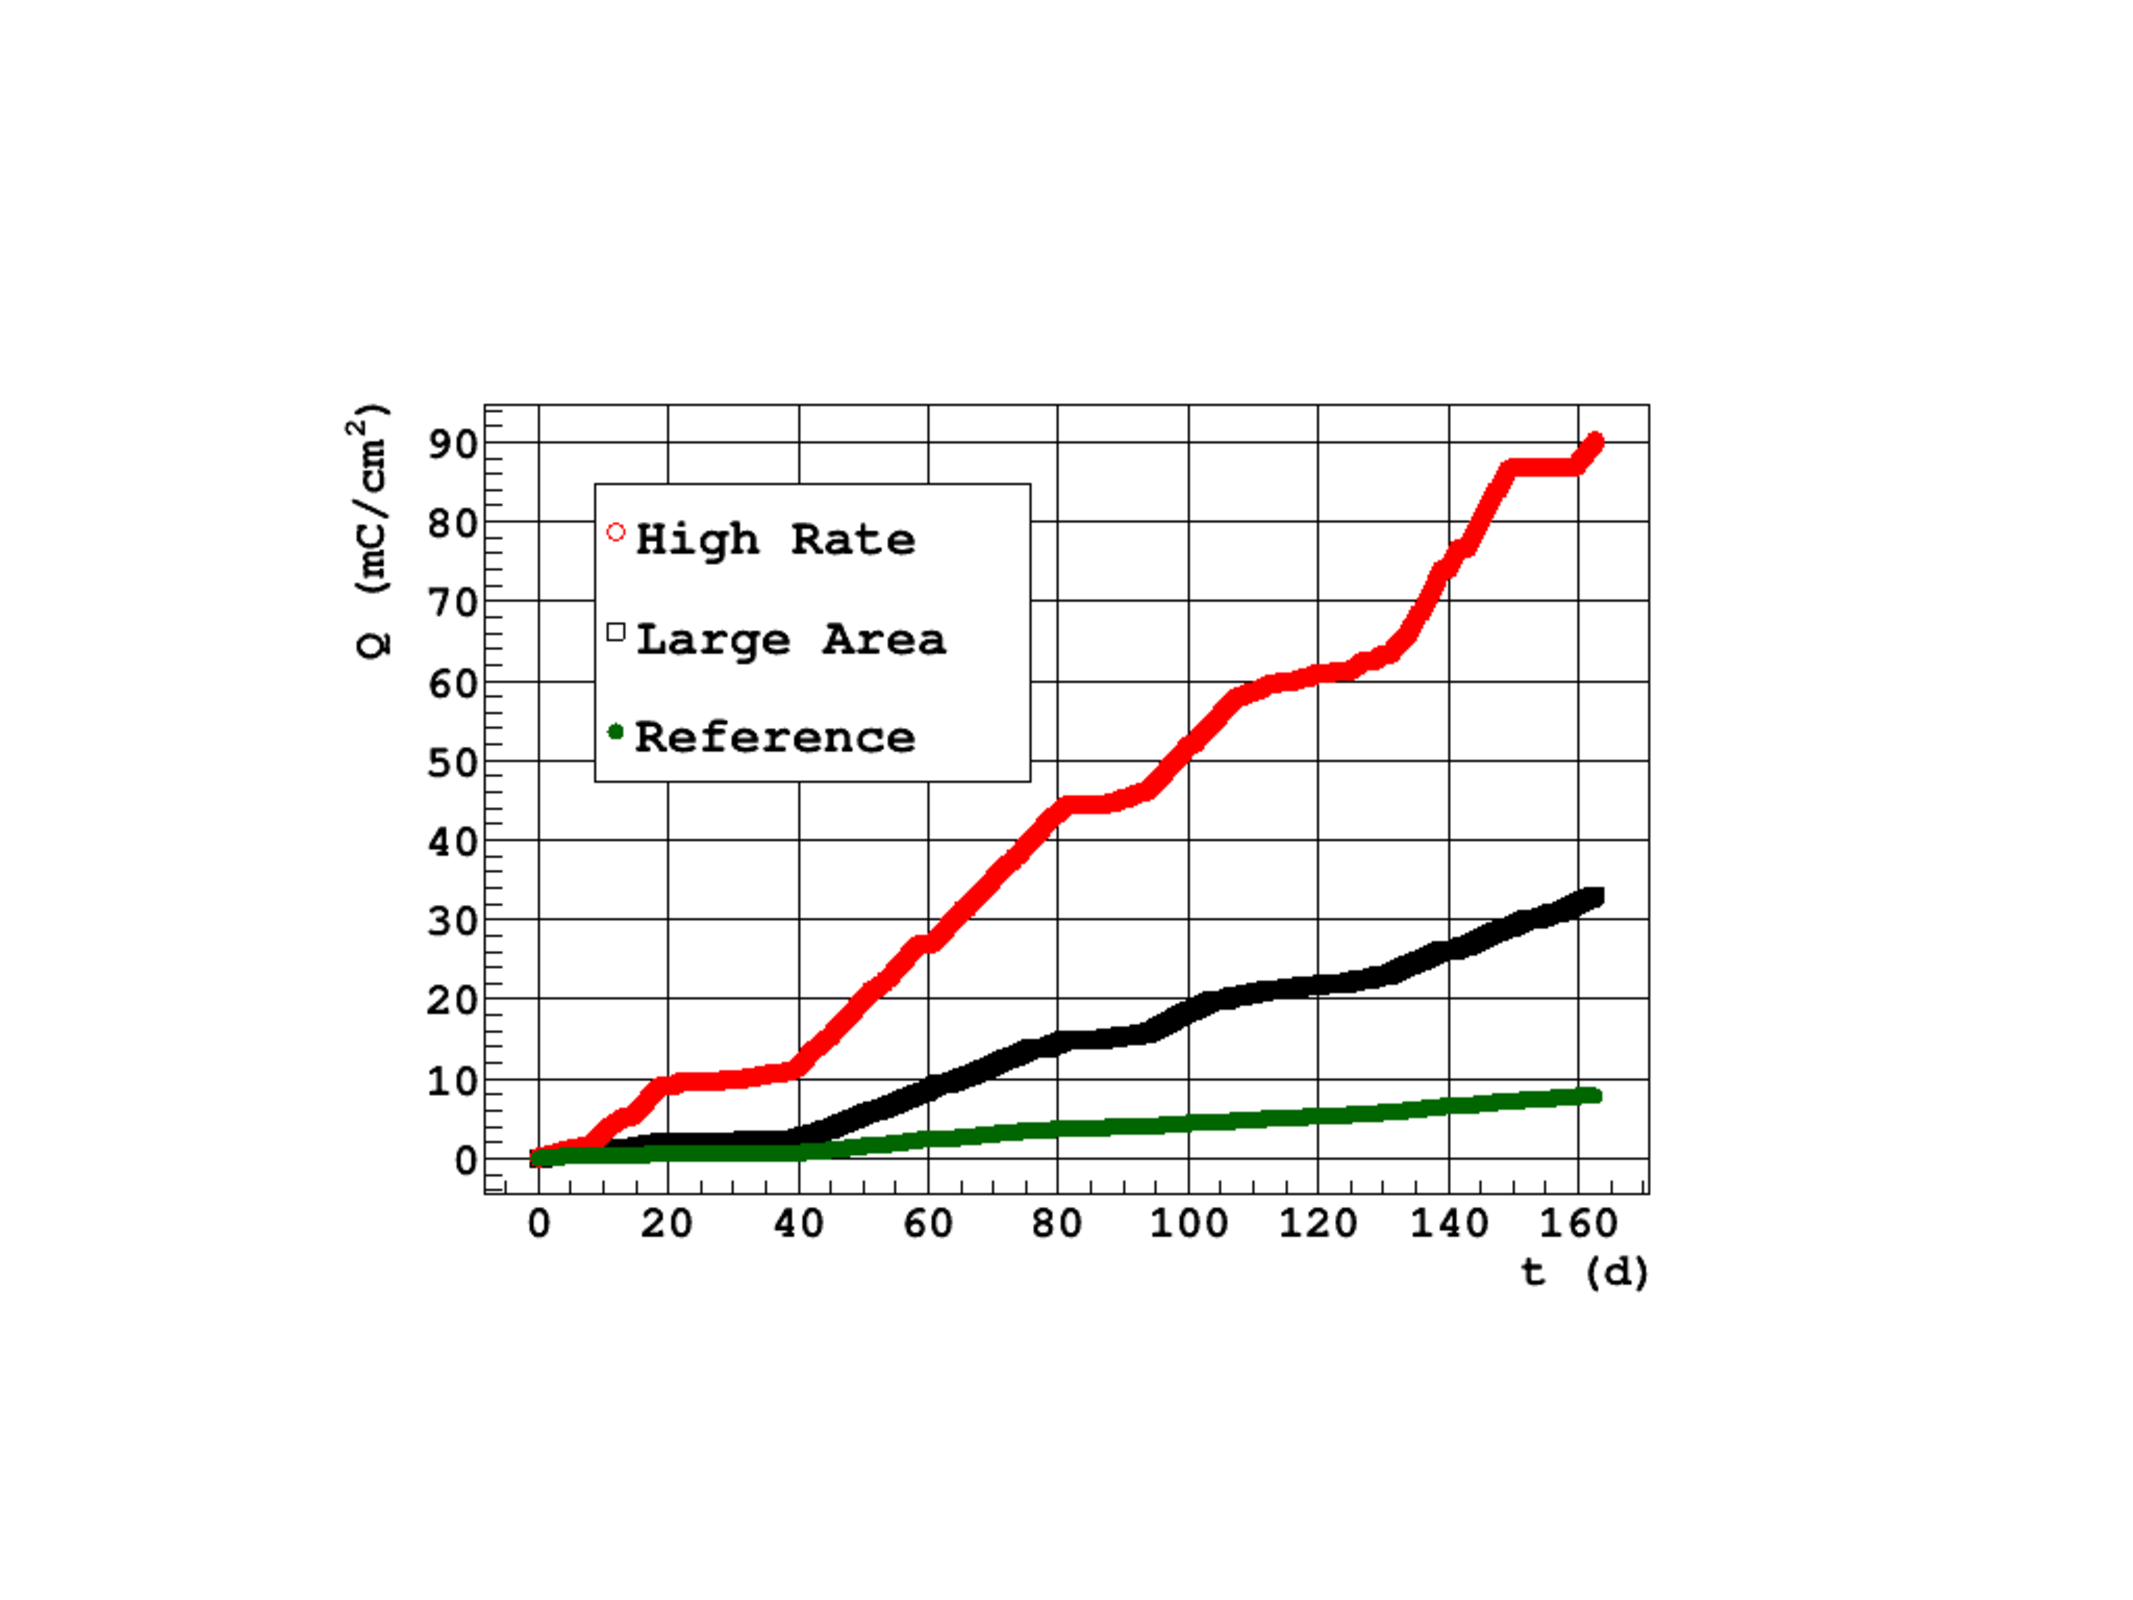
\includegraphics[width=0.7\textwidth] {Figures/Muon/microrwell-dose-GIF.pdf}
\caption{Dose accumulated at the GIF++. The GE11 size detector is labelled \textit{Large Area} and has accumulated about 23 mC/cm$^2$, equivalent to more than 100 years of operation at HL-LHC conditions. }
\label{fig:urwell-int-dose}
\end{figure}


\subsection{The double-resistive layer detector}
\label{sec:DRL}
%
As discussed in \cite{micro-RWELL}, the $\mu$RWell based on the single-resistive layout characterized by a 2-D evacuation scheme (with grounding all around the edge of the detector surface) suffers at high particle fluxes of a non-uniform response over its surface.
This is due to  the resistance ($\Omega_{single}$) seen by the current generated by the incident radiation that depends on the distance to ground (for the definition of $\Omega$ see the appendix B of the cited reference).\\
% 
\begin{figure}
	\begin{center}
%		\includegraphics[scale=0.5]{uRWELL_doublelayer}
       \caption{Double-resistive layout for high rate operation.}
        \label{resistive-stage2}
        \end{center}
\end{figure}
%  
In order to get rid of such a limitation a double-resistive layout (fig.~\ref{resistive-stage2}) has been proposed: the first DLC film, in contact with the amplification stage of the detector, is connected to a second DLC film by means of a matrix of through-vias and then grounded with a second matrix of through-vias to the underlying readout electrodes.\\
%
In this way a sort of discrete 3D-current evacuation layout is obtained and the  $\Omega_{double}$ seen by the current is minimized with respect to the single-resistive layer scheme just for geometry and Ohm's law considerations.\\
Comparing a 50$\times$50 cm$^2$ single-resistive detector with a double-resistive detector of the same size, but with a through-vias density of 1 cm$^{-2}$, and assuming the same surface resistivity of the DLC films for both devices, a $\Omega_{double}$/$\Omega_{single}$ ratio (and correspondingly the ratio between the voltage drop $\Delta$V$_{double}$/$\Delta$V$_{single}$) of the order of 1/10 is obtained. As a consequence an improvement of a factor of ten of the rate capability could be achieved with the double-resistive technology.\\
%
\begin{figure}[h]
	\begin{center}
		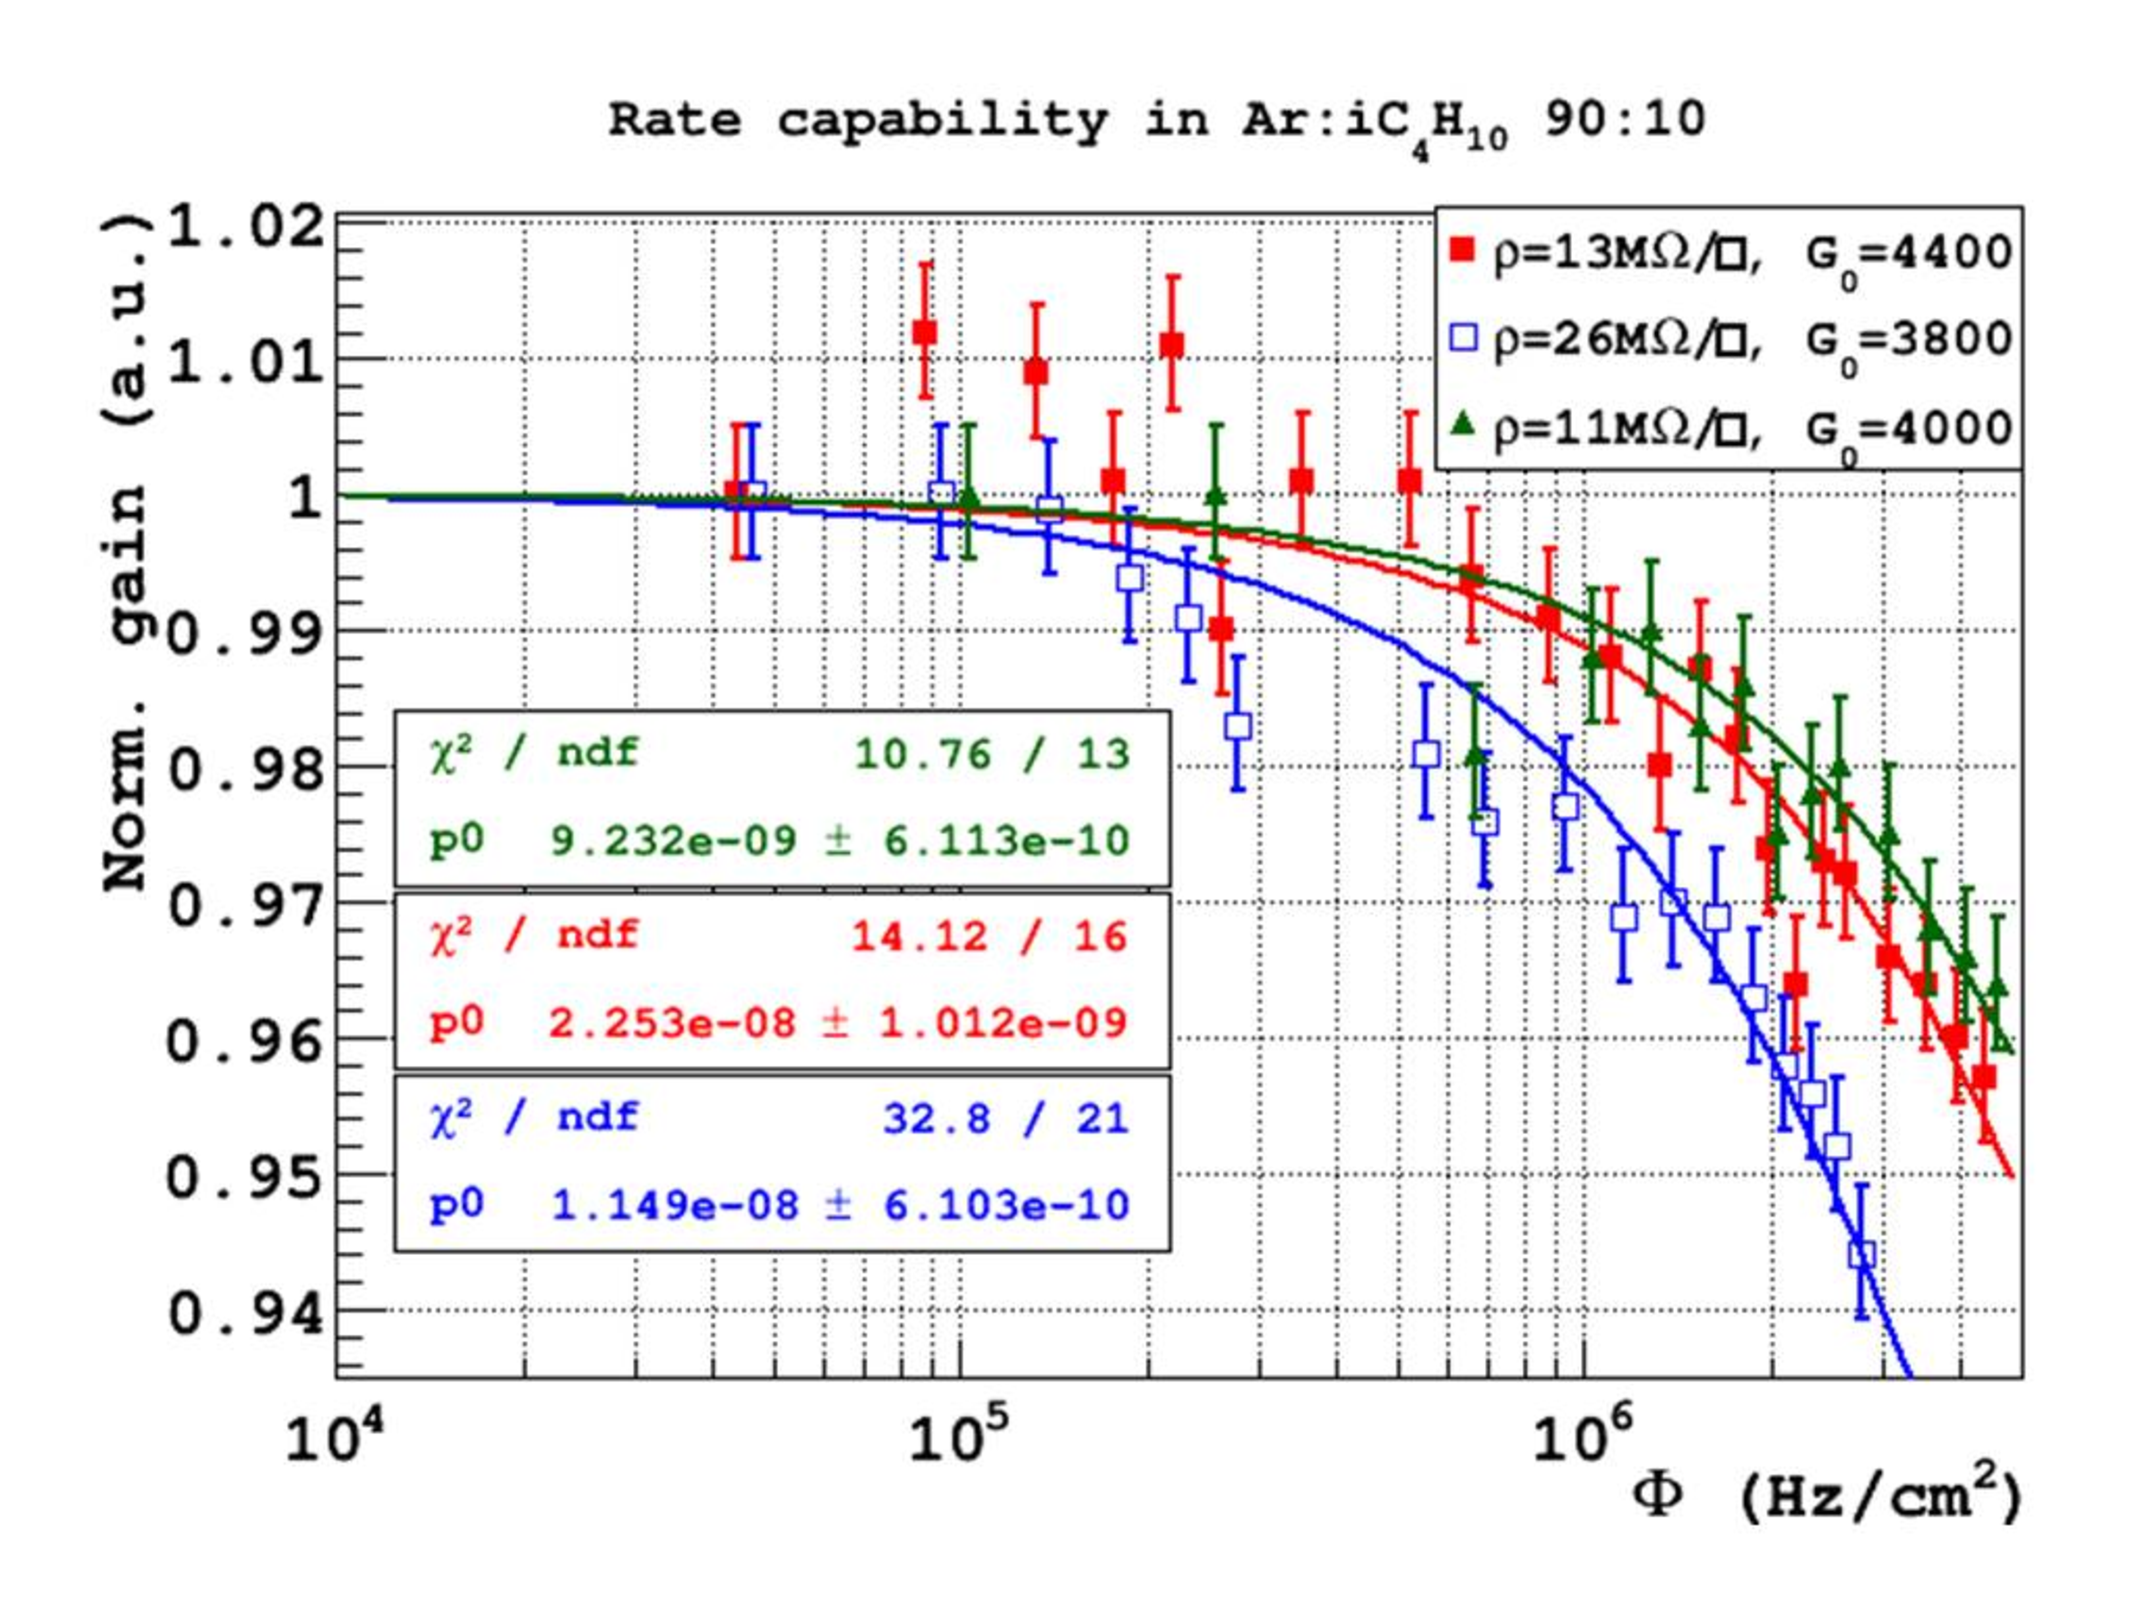
\includegraphics[scale=0.35]{Figures/Muon/microrwell-ariso-ratecapa-double-layer.pdf}	
        \caption{Normalized gain for double-layer prototypes: 11~M$\Omega/\Box$ (green triangles), 13~M$\Omega/\Box$ (red full square) and 26~M$\Omega/\Box$ (blue empty sqaure)}
    	\label{ratecapa-double}
	\end{center}
\end{figure}
%
The rate capability for different DLC-film resistivity 10$\times$10 cm$^2$ double-layer prototypes with 1 cm$^{-2}$ through-vias grounding density (pitch) has been measured with 5 mm diameter collimated X-ray beam. In this case the results, shown in fig.\ref{ratecapa-double}, even though performed with local irradiation are  practically equivalent to those obtained with global irradiation.
%

\subsection{Applications for a Muon detection system for a CepC experiment}
\label{section:Muon-detector}
%
The $\mu$RWell technology, especially in its \textit{low-rate} version, is a mature solution, with whom single detectors of a 0.5 m$^2$ have been realised and succesfully operated in the laboratory as well as in test beams. They can withstand particle rates up to a few tens of kHz/cm$^2$, providing a position resolution as good as $\sim$60 $\mu$m wuth a time resolution of 5-6 ns. Moreover the $\mu$RWell technology is a robust solution, intrinsically safer against sparks than, for example, the widely used GEM detectors. In comparison with the GEM detectors the construction is much simpler, involving no stretching of the kapton foils and only one amplification stage instead of the three stages of the triple-GEM solution. This makes the cost of a $\mu$RWell detector typically less than half the cost of a triple-GEM detector of the same size and the same strip pitch. A few industries have already started collaborating and producing some of the components of the $\mu$RWell detectors, and in a very short time, all the needed $\mu$RWell detector components will be produceable by industry.
This technology could therefore be very effectively used for realizing a muon detection system for CepC. In particular this detector, which would have dimensions of a few thousand m$^2$ could be realised by using tiles of $\mu$RWell detectors of a size 50x50 cms$^2$. Each tile woud have a relatively small gas volume of $\sim$1 l. This would make the whole muon detector very modular with components bought directly from industry. The needed assembly and quality control of the $\mu$RWell detectors could then be efficiently realised by the collaborating institutes.
A CepC muon detector made of $\mu$RWell tiles could consist of the three successive muon stations, each equipped with a couple of layers of $\mu$RWell detectors in order to provide a very precise, of the order of 200$\mu$m, position resolution on the coordinates of a muon track. The time resolution would be 5-6 ns. This precise position resolution, together with the three stations, would allow to have an independent muon tracking that could then also be associated back to the tracks measured by the central tracker. This would make for a very robust and efficient muon detection system. A  muon trigger system, albeit probably not essential for a CepC detector, could be easily implemented.
A similar muon detection scheme, could be envisaged also for a SppC detector, eventually using the \textit{high-rate} $\mu$RWell detectors in the regions where the highest particle rates are foreseen.



